% !TEX root = ../YourName-Dissertation.tex

\chapter{Direct Measurement of the Neutrino Mass with Project 8}

\section{Introduction}

A promising technique for direct measurements of the neutrino mass beyond the projected limit of the ongoing KATRIN experiment is tritium beta-decay spectroscopy with an atomic tritium source \cite{direct_meas_nu_mass}. Atomic tritium, combined with a large-volume, high-resolution energy measurement technique, is capable of measuring the neutrino mass with sensitivity below the 50~meV limit allowed by neutrino oscillations. 

Cyclotron Radiation Emission Spectroscopy or CRES is a high-resolution energy measurement technique compatible with atomic tritium production and storage that can enable the next-generation of neutrino mass direct measurement experiments \cite{p8originalcres}. The Project 8 collaboration is currently engaged in a program of research and development (R\&D) aimed at developing the technology necessary for a 40~meV sensitivity measurement of the neutrino mass using CRES and atomic tritium \cite{p8snowmass2022}.

In Section \ref{sec:chap3-cres-and-p8} we provide and introduction to the basics of the CRES technique as well as the goals of the Project 8 experiment. Additionally, we sketch out the phased experiment development plan being implemented by Project 8 to build towards a next-generation neutrino mass experiment.

In Section \ref{sec:chap3-phaseII} we give a brief overview of Phase II of the Project 8 experiment \cite{p8prc2023,p8prl2023}, which completed early in 2023. Although the bulk of the work presented in this thesis is relevant to designs of future Project 8 experiments, a description of the work in Phase II provides useful context for the rest of the work.

In Section \ref{sec:chap3-phaseIII-antenna-arrays} we introduce a CRES measurement concept based on antenna arrays \cite{p8jugaad}, which could be the basis for the ultimate Project 8 neutrino mass experiment. A significant portion of the R\&D efforts of Project 8 in Phase III were directed towards simulating and modeling this experimental concept in order to understand the achievable sensitivity to the neutrino mass.

Lastly, in Section \ref{sec:chap3-freq-choice-and-pilot-scale} we introduce conceptual designs of pilot-scale experiments that combine atomic CRES with a large-volume CRES detection technique. This includes a design concept for an antenna array based experiment, but also a design for a resonant cavity based experiment. Resonant cavities are discussed in more depth in Chapter \ref{chap:cavity} and have become the preferred choice for future CRES experiments in Project 8 over antenna arrays.

\section{Cyclotron Radiation Emission Spectroscopy and Project 8}
\label{sec:chap3-cres-and-p8}

\subsection{Cyclotron Radiation Emission Spectroscopy --- CRES}

Of the standard physical quantities the one that can be measured with the highest precision is time and the inversely related quantity frequency. In fact it is often advantageous to convert measurements of other physical quantities like mass or length into frequency measurements due to the digital nature of frequency measurements that make them immune to many sources of noise. Atomic clocks, which operate by measuring the frequencies of various atomic transitions, have been used to measure time with astounding relative uncertainties of $10^{-18}$~seconds. The extreme precision possible with frequency measurements is often summarized using the a quote from the Physicist Arthur Schawlow who said advise his students to "Never measure anything but frequency!". 

Neutrino mass measurements using tritium beta-decay require us to measure a perturbation of the 18600~eV tritium endpoint to precisions as low as 0.1~eV, therefore, a spectroscopic technique with extremely high resolution is required for this measurement. Part of the reason that frequency measurements are capable of such high resolutions is that they are essentially counting measurements, which average the number of oscillations of a physical system over time. By observing a rapidly oscillating system over a sufficient length of time one can obtain essentially arbitrary precision on a frequency limited only by the time available for measurement and the SNR of the system.

In order to perform frequency-based high-resolution spectroscopy of the tritium beta-decay spectrum one needs to translate the kinetic energy of the electron into a frequency. The simplest way to accomplish this is to place a gaseous supply of tritium into a magnetic field. When one of the atoms decays the resulting electron will immediately begin to orbit around a magnetic field line at the cyclotron frequency which is proportional to its kinetic energy (see Figure \ref{fig:chap3-cres-cartoon}). The acceleration caused by the orbit leads to the emission of cyclotron radiation that can be detected using an array of antennas or a different RF sensor such as a resonant cavity. The frequency of the radiation gives the electron's kinetic energy, which is used to build the beta-decay spectrum and measure the neutrino mass. The name for this measurement technique is Cyclotron Radiation Emission Spectroscopy or CRES.

\begin{figure}[htbp]
    \centering
    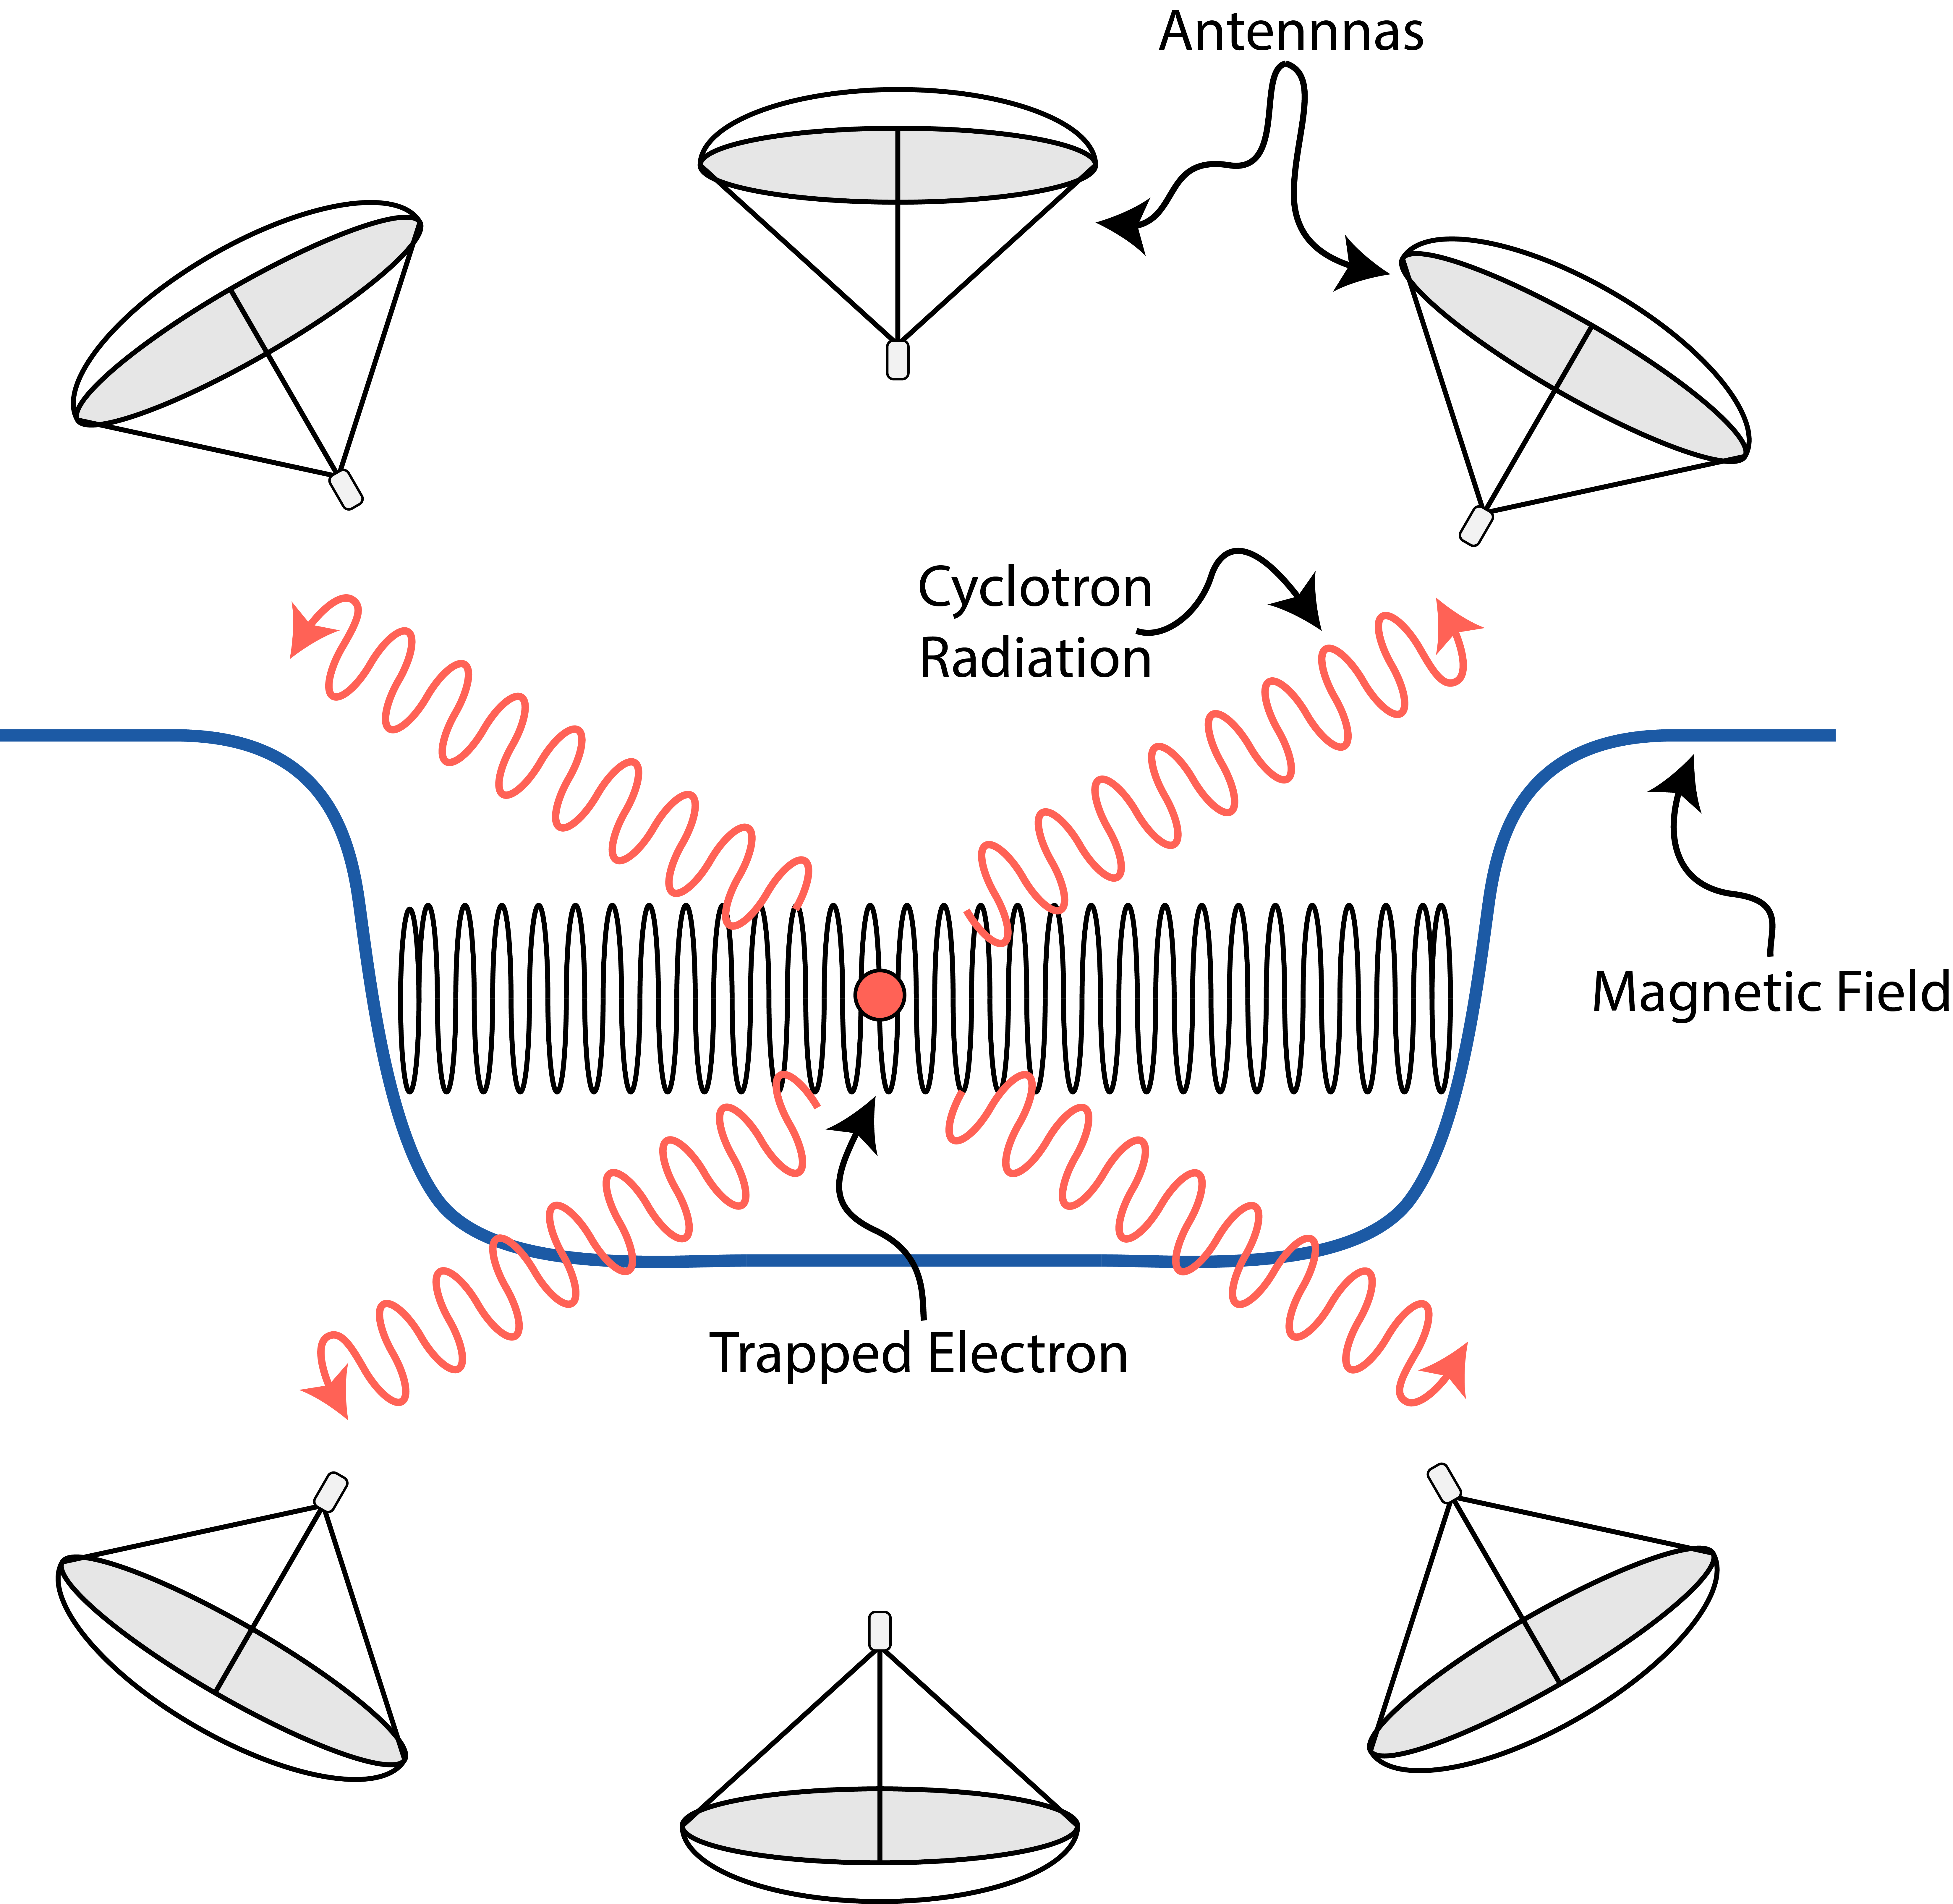
\includegraphics[width=0.5\textwidth]{figs/Chapter-3/230303_cres_cartoon.png}
    \caption{A cartoon illustration of the CRES technique. An electron is contained in a magnetic trap so that it's cyclotron radiation can be detected by an array of antennas. Detecting the cyclotron radiation allows us to measure its cyclotron frequency and determine its kinetic energy.}
    \label{fig:chap3-cres-cartoon}
\end{figure}

For non-relativistic particles the cyclotron frequency is only a function of the charge-to-mass ratio of the particle, however, from the relativistic form of the cyclotron frequency
\begin{equation}
    f_c = \frac{qB}{2\pi m_e\gamma}=\frac{1}{2\pi}\frac{qB}{m_e+E_\mathrm{kin}/c^2},
    \label{eq:chap3-cyclotron-freq}
\end{equation} 
one can see that the kinetic energy ($E_\mathrm{kin}$) of the electron is directly proportional to the inverse of the cyclotron frequency ($f_c$). Electrons with kinetic energies of 18.6~keV are in the weakly relativistic regime with $\beta=\frac{v}{c}=0.263$ and $\gamma=1.036$.

The required frequency resolution needed for neutrino mass measurement can be obtained by differentiating Equation \ref{eq:chap3-cyclotron-freq},
\begin{equation}
    \frac{df_c}{dE_\mathrm{kin}} = \frac{1}{2\pi}\frac{-qBc^2}{\left(m_ec^2+E_\mathrm{kin}\right)^2},
\end{equation}
from which we can obtain the relationship between fractional differences in energy and frequency,
\begin{equation}
    \frac{df_c}{f_c}=\frac{1-\gamma}{\gamma}\frac{dE_\mathrm{kin}}{E_\mathrm{kin}}.
\end{equation}
Therefore, an energy precision of 1~eV for an 18.6~keV electron requires a frequency precision of approximately 2~ppm.

The minimum observation time required to achieve this resolution can be estimated using the uncertainty principle as formulated by Gabor. Electron's from tritium beta-decay experience random collisions with the background gas particles, which limits the uninterrupted radiation lifetime. The time between collision events, referred to as track length in the context of CRES measurements, is an exponentially distributed variable. Differences in the track lengths of a population of mono-energetic electrons leads to uncertainty or broadening in the distribution of measured frequencies proportional to the mean track length, $\tau_\lambda$. The resulting frequency distribution has a Lorentizan profile, whose width is given by the Gabor limit,
\begin{equation}
    \tau_\lambda\Delta f_c=\frac{1}{2\pi}\implies\Delta f_c=\frac{1}{2\pi\tau_\lambda}.
\end{equation}

The cyclotron frequency for a 18.6-keV electron in a 1~T field is approximately 27~GHz, from which one can estimate the minimum observation time for 2~ppm frequency resolution at approximately 3~$\mu$sec. The Gabor limit is not the true lower bound on the frequency resolution for a CRES signal, since it is based on the details of the Fourier representation of a time-series with a fixed length. If one takes the approach of fitting the CRES signal in the time-domain, then one finds that the limit on frequency precision is given by the Cram\'{e}r-Rao lower bound (CRLB), which depends on both the track length as well as the SNR. In general, the CRLB allows for better precision on the cyclotron frequency, however, the Gabor limit provides an illustrative limit with the correct order of magnitude.  

\begin{figure}[htbp]
    \centering
    \includegraphics*[width=0.75\textwidth]{figs/Chapter-3/230628_bathtub_trap.png}
    \caption{\label{fig:chap3-bathtub-trap}An illustration of an electron in a bathtub magnetic trap generated by two well-separated coils.}
\end{figure}

Ensuring that an electron remains under observation long enough so that it's frequency can be properly measured requires a magnetic trap. A magnetic trap is a local minimum in a background magnetic field generated an appropriate configuration of electromagnetic coils. Since magnetic fields can do no work, there is no danger of the magnetic trap affecting the kinetic energy electron after it is emitted from the beta-decay. One common approach to creating a magnetic trap is the "bathtub" trap configuration, which in it's simplest form consists of two high magnetic field pinch coils aligned on a central axis that are well separated (see Figure \ref{fig:chap3-bathtub-trap}). This configuration produces a trap with a flat uniform bottom and relatively steep walls, which is ideal for CRES measurements. 

Electrons produced in the trap oscillate back and forth between the trap walls at a frequency that depends upon the pitch angle, unless they are produced with pitch angles too small to be contained in the trap. Pitch angle is defined as the angle between the component of the electron's velocity perpendicular to the magnetic field and the component parallel to the magnetic field,
\begin{equation}
    \tan{\theta}=\frac{v_\perp}{v_\parallel}.
\end{equation}
The axial motion of the electron leads to variation in the cyclotron frequency due to the changing value of the magnetic fields. This leads to frequency modulation that generate sidebands in the cyclotron radiation spectrum. Resolving these sideband frequency components is necessary for a complete reconstruction of the CRES signal in the experiment.

Electrons trapped in a cylindrically symmetric trap have three primary components of motion (see Figure \ref{fig:chap3-trapped-electron-motion}).
\begin{figure}[htbp]
    \centering
    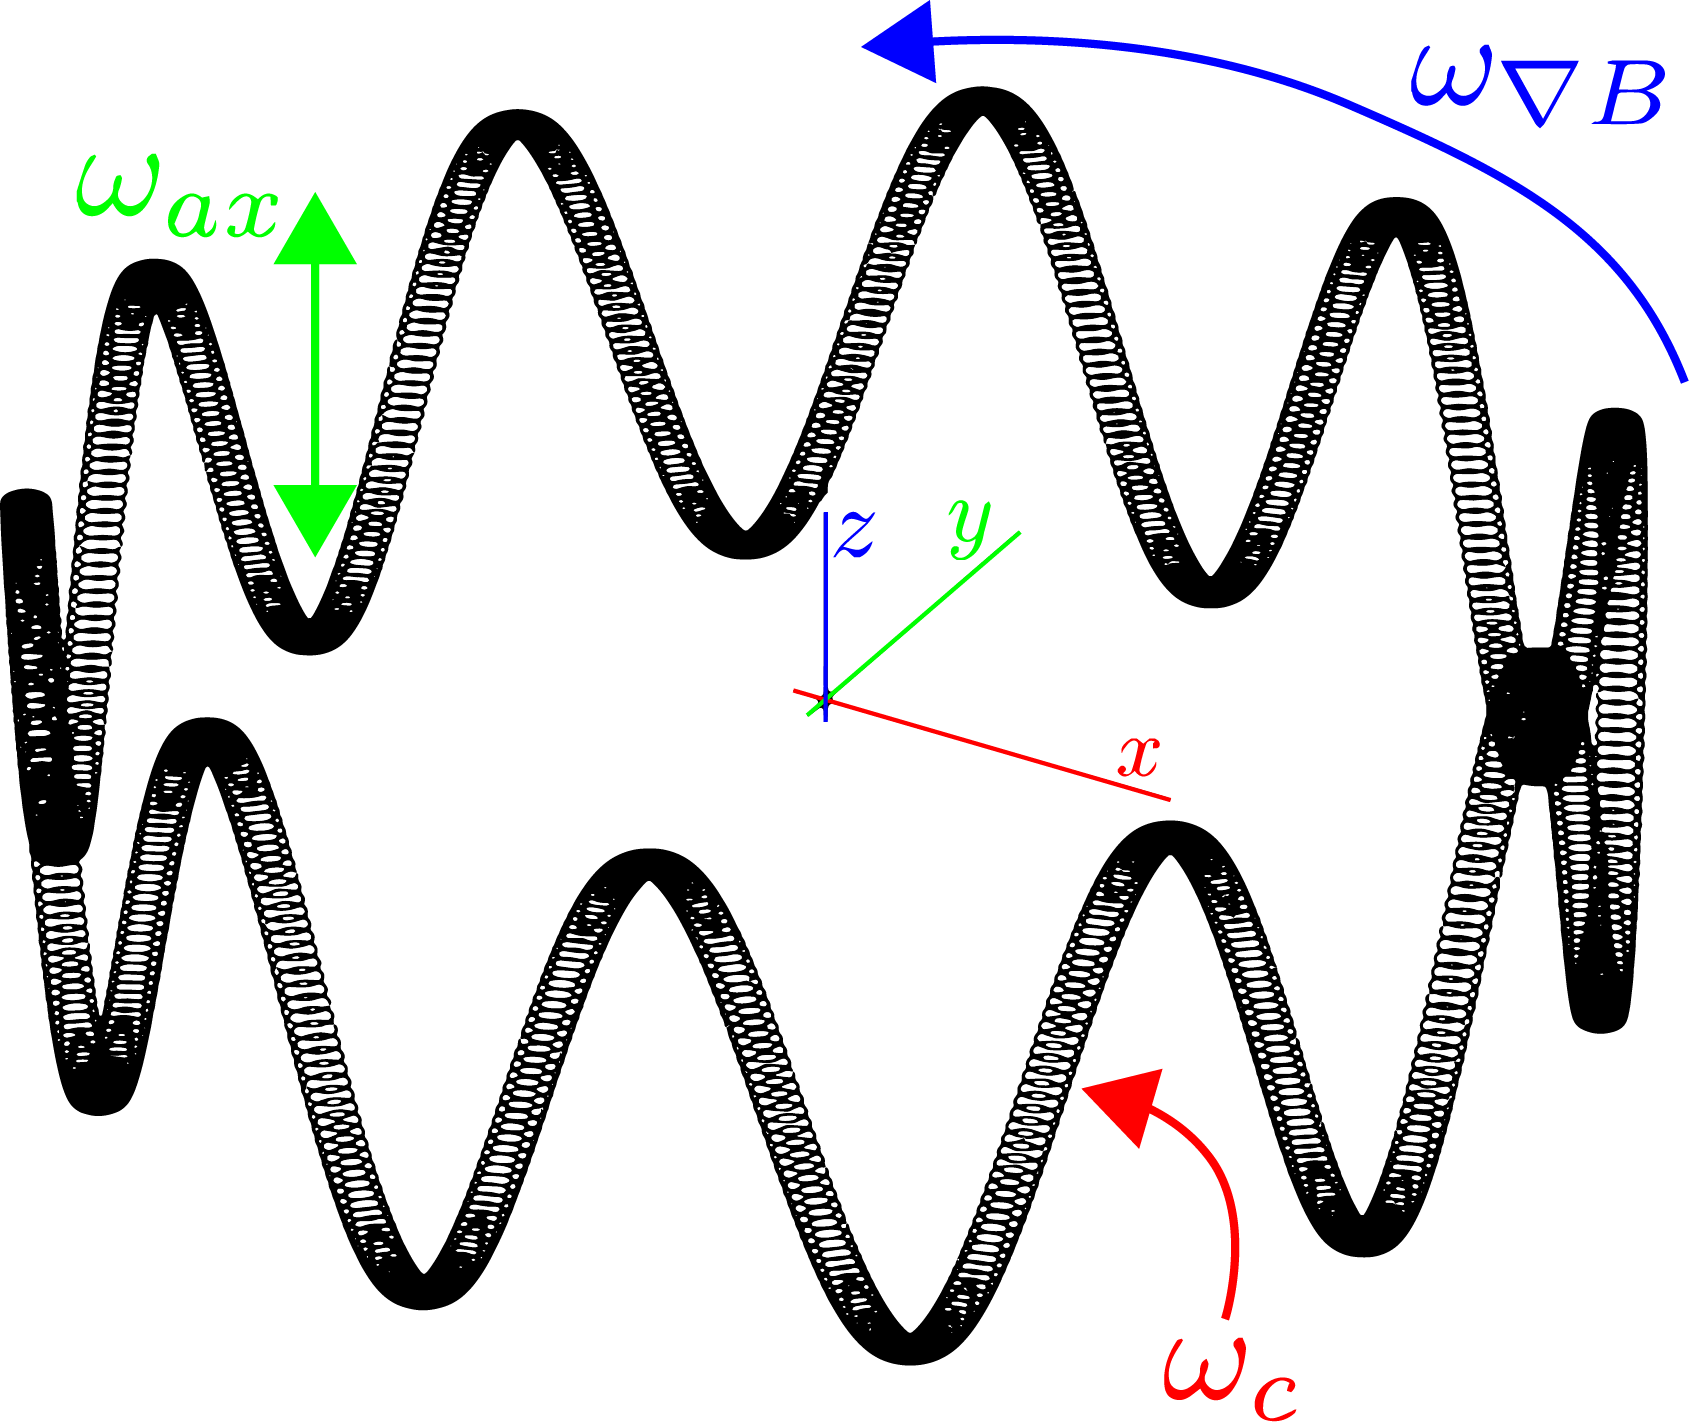
\includegraphics[width=0.5\textwidth]{figs/Chapter-3/230511_trapped_motion.png}
    \caption{A plot of the main components of an electron's trajectory in a cylindrically symmetric trap.}
    \label{fig:chap3-trapped-electron-motion}
\end{figure}
The dominant component, typically with the highest frequency, is the electron's cyclotron orbit, which encodes information on the electron's kinetic energy. Axial motion from the electron's pitch angle leads to frequency modulation but also a shift in the average magnetic field experienced by an electron. This leads to a correlation between the kinetic energy of the electron and the pitch angle depending on the particular shape of the magnetic trap, which can negatively impact energy resolution. To reduce this correlation one must engineer the trap to have a flat bottom with very steep wall both of which are more easily achieved with a small aspect ratio bathtub trap. Radial gradients in the trap oftentimes leads to a third component of motion called grad-B drift. The equation for the drift velocity is
\begin{equation}
    \mathbf{v}_{\nabla B} = \frac{m_e v_\perp^2}{2qB}\frac{\mathbf{B}\times\nabla B}{B^2}.
\end{equation}
These additional components of motion all influence the shape of the CRES signal so modeling their effects is critical to proper measurement of the kinetic energy.

The total power of the radiation emitted by an electron in a free-space environment is given by the Larmor equation
\begin{equation}
    P(\gamma, \theta_p)=\frac{1}{4\pi\epsilon_0}\frac{2}{3}\frac{q^2\omega_c^2}{c}(\gamma^2 - 1)\sin^2{\theta_p},
\end{equation}
where $\omega_c$ is the cyclotron frequency multiplied by $2\pi$ and $\theta_p$ is the pitch angle to distinguish it from the spherical angle coordinate. A single electron with a $90^\circ$ pitch angle and 18.6~keV of kinetic energy in a 1~T magnetic field emits a total radiation power of 1.2~fW, which is quite small compared with typical RF systems, furthermore, one is typically only able to receive a fraction of this total power with an antenna or other detection system. Therefore, RF systems in CRES experiments must be operated at cyrogenic temperatures to limit the noise power such that adequate SNR can be achieved for signal detection and reconstruction. Alternatively, longer tracks enable detection of weaker signals due to the increase in the total signal energy available for the detection algorithm.

\subsection{The Project 8 Collaboration}

The Project 8 collaboration is a group of institutions in the United States and Germany aiming to measure the neutrino mass by developing a novel spectrometer technology based on CRES. In the ultimate Project 8 experiment the CRES technique will be used to measure the beta-decay spectrum using a large source of atomic tritium sufficient to achieve the required statistics in the last $O(10)$~eV of the decay spectrum. Project 8 is targeting a neutrino mass sensitivity below 50~meV, which exhausts the range of possible neutrino masses under the inverted hierarchy and is a factor of four less than sensitivity projections for the ongoing KATRIN experiment.

Project 8's proposed experiment requires the development of two novel technologies: the production and trapping of a source of atomic tritium on cubic-meter scales and technology to enable CRES measurements of individual electrons in the same volume. 

\subsubsection*{Atomic Tritium}

Previous measurements of the tritium beta-decay spectrum for neutrino mass measurements have all relied on a sources of molecular tritium for their measurements due to the numerous practical and technical challenges associated with the production and storage of hydrogen isotopes.

\begin{figure}[htbp]
    \centering
    \includegraphics*[width=0.5\textwidth]{figs/Chapter-3/atmol2.pdf}
    \caption{\label{fig:chap3-atomic-vs-mol-final-state-spectra} A plot of the final state distributions of atomic and molecular tritium. The final state distribution provides the primary contribution to the width of the molecular spectrum whereas thermal doppler broadening is responsible for the width of the atomic spectrum.}
\end{figure}

To produce atomic hydrogen one must supply sufficient energy to the tritium molecule to break the molecular bond between. Common approaches to this include the use of hot coaxial filament atom crackers as well as plasma atom sources. Both approaches heat the tritium atoms to temperatures $>2500$~K, which must then be cooled to temperatures on the order of a few~mK so that the tritium atoms can be trapped. Cooling the atoms requires the construction of a large tritium infrastructure and cooling system that can supply a source of cold atoms to the trap. 

Once cold tritium atoms are produced they cannot make contact with any surfaces to avoid recombination of the atoms to molecules. Therefore, a magnetic trap is required to store the atoms for a sufficient length of time that they have a chance to decay before escaping the trap. Trapping the atoms at this scale requires the construction of a large and complex magnet system that must be cooled to cryogenic temperatures to avoid heating of the atoms, which leads to their escape from the trap.

The significant experimental complexity caused by atomic tritium makes a molecular source the obvious choice from practical considerations. However, the drawback of molecular tritium for neutrino mass measurement is the irreducible broadening in the electron's kinetic energy due to the final state spectrum of molecular tritium (see Figure \ref{fig:chap3-atomic-vs-mol-final-state-spectra}). The broadening of the final state spectra has a RMS amplitude of 436~meV caused by variation in the final vibrational state of the daughter molecule. For atomic tritium the primary sources of broadening in the final state spectrum are magnetic hyperfine splittings ($O(10^{-5})$~eV) and thermal Doppler broadening caused by the motion of the trapped atom. For atomic tritium at a temperature of 1~mK thermal broadening is the dominant contribution, providing about 1~meV RMS of broadening to the electron's kinetic energy.

The larger energy broadening with molecular tritium leads to an irreducible statistical uncertainty that limits the achievable sensitivity to approximately 100~meV at 90\% confidence. For previous direct measurements of the neutrino mass this uncertainty is an insignificant contribution to the overall uncertainty budget, however, for experiments like Project 8 atomic tritium is a key component to the success of the experiment.

\subsubsection*{CRES for Neutrino Mass Measurement}

Several promising features of the CRES technique make it a particularly attractive choice for a next generation neutrino mass measurement experiment. For example, with a CRES experiment the volume of the source gas can be the same as the volume of the CRES spectrometer. This is due to the fact that CRES is a remote-sensing technique that can observe the energy of the electron without altering its trajectory or directly interacting with the electron. Given that tritium gas is transparent to cyclotron radiation the kinetic energies of electrons can be measured with an appropriate sensing technology, such as a cavity or antenna array, located directly outside the atom trapping volume. 

The current state-of-the-art tritium beta-decay spectroscopy experiment, KATRIN, utilizes the magnetic adiabatic collimation with an electrostatic filter (MAC-E filter) technique to measure the beta-decay spectrum of molecular tritium. In this approach, a source of molecular tritium is located outside of the spectrometer. When a beta-decay occurs the electron must exit the tritium source and travel through the MAC-E filter before it can be detected on the other side of the filter using a charge sensor. With this approach the measurement statistics are limited by the transverse areas of the tritium source and MAC-E filter due to the need to travel through the detector without scattering. This scaling is less favorable than the volumetric scaling that one has with CRES due to the ability to co-locate source and detector.

Another promising aspect of the CRES technique is the inherently high precision of frequency based measurements. The endpoint of the molecular tritium beta-decay spectrum is approximately 18.6~keV, which dwarfs the neutrino mass scale of $<1$~eV/$\rm{c}^2$ by at least a factor of $10^5$. Measuring the effect of such a small mass on a high energy electron requires excellent energy resolution. Since frequency measurements are essentially counting measurements they are intrinsically quite accurate due to the ability to measure the cyclotron frequency by effectively averaging over millions of cyclotron orbits. Using off-the-shelf RF components its is possible to achieve part-per-million accuracy on the kinetic energy with the CRES technique.

A final aspect of the CRES technique that is attractive for a next-generation experiment is the relative immunity to backgrounds. Since CRES operates via non-destructive measurements of the electron's cyclotron frequency potential sources of background electrons are effectively filtered out by limiting the frequency bandwidth of the measurement. The fiducial volume of the experiment is free from any surfaces that could introduce stray electrons and electrons from sources outside the fiducial volume can be prevented from entering the experiment.

\subsubsection*{Neutrino Mass Sensitivity Goals}

Project 8's ultimate goal is to combine CRES with atomic tritium to measure the neutrino mass with 40~meV sensitivity at the 90\% confidence level (see Figure \ref{fig:chap3-p8-nu-mass-goal}).
\begin{figure}[htbp]
    \centering
    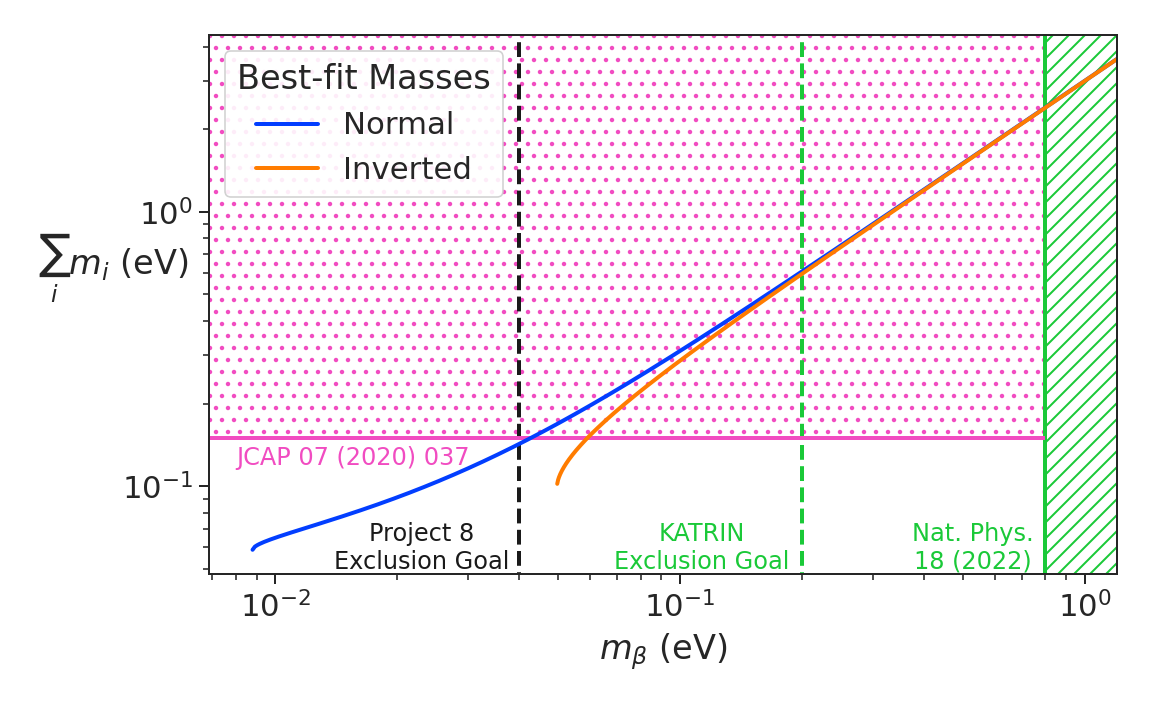
\includegraphics[width=0.7\textwidth]{figs/Chapter-3/230303_sum_nu_mass_vs_m_beta_with_exclusion_and_goal.png}
    \caption{Neutrino mass exclusion plot including limits from cosmological measurements and the KATRIN experiment. Allowed ranges for neutrino masses under the normal and inverted hierarchies are shown as the blue and orange lines respectively. The black dashed line shows Project 8's goal neutrino mass sensitivity for the Phase IV experiment.}
    \label{fig:chap3-p8-nu-mass-goal}
\end{figure}
This sensitivity is sufficient to fully exhaust the range of allowable neutrino masses under the inverted neutrino mass ordering regime and is approximately an order of magnitude less than the projected final sensitivity of the KATRIN experiment. Excluding the full neutrino mass parameter space would require a sensitivity an order of magnitude lower than what is proposed by Project 8, which would require an experiment whose size and complexity are currently well beyond proposals for the next-generation of neutrino mass direct measurement experiments.

\subsection{Project 8 Phased Development Plan}

Reaching 40~meV sensitivity will require the simultaneous development and eventually combination of two novel technologies. The first is the technology required to supply a source of atomic tritium of the appropriate size, density, purity, and temperature along so that the atoms can be trapped and their beta-decays measured in the spectrometer. The second is a CRES measurement technology that is both compatible with the tritium atom trap and is capable of reconstructing CRES events with sufficient energy resolution to achieve the required sensitivity.

\begin{figure}[htbp]
    \centering
    \begin{subfigure}{0.725\textwidth}
        \includegraphics*[width=\textwidth]{figs/Chapter-3/sensitivity_vs_exposure_curve.pdf}
    \end{subfigure}
    \begin{subfigure}{0.67\textwidth}
        \includegraphics*[width=\textwidth]{figs/Chapter-3/sensitivity_vs_density_curve.pdf}
    \end{subfigure}
    \caption{Sensitivity calculations for a cavity based CRES experiment that demonstrate the neutrino mass measurement goals of the Project 8 collaboration throughout the phased development plan. The blue tinged curves indicate molecular tritium sources and the red tinged curves indicate atomic tritium sources. In the current plan Phase III contains two tritium experiments. The first is the Low-frequency Apparatus (LFA) which is a molecular tritium experiment and the second is the atomic tritium pilot-scale experiment that ends Phase III. The sensitivity of these experiments is primarily a function of statistics, however, there is a critical density beyond which CRES electrons do not have enough time to radiate between collisions for a high-resolution frequency measurement leading to worse sensitivity. }
\end{figure}

These technologies require a significant up-front research and development (R\&D) investment to build-out the required capabilities for a 40~meV CRES experiment. Therefore, Project 8 is following a phased experiment plan in which incremental progress can be made towards the ultimate goal of a 40~meV neutrino mass measurement with CRES.

\subsubsection*{Phase I and II: Proof of Principle and First Tritium Measurements}

The earlier phases of the Project 8 experiment, Phase I and II, were focused on demonstration and development of the CRES technique itself as well as a proof-of-principle measurement of the neutrino mass using the CRES technique.

In Phase I, Project 8 performed a proof-of-principle measurement of the $^{83m}\rm{Kr}$ spectrum using CRES, which marked the first ever energy spectrum measurement with CRES. The experiment included all of the main components expected for the full-scale version of the experiment. An electron source consisting of a gas of $^{83m}\rm{Kr}$ was supplied to a waveguide gas cell constructed out of a segment of WR-42 waveguide and sealed with Kapton windows at the top and bottom. A magnetic trapping region was created in the waveguide cell using a single electromagnetic coil wrapped around the waveguide which provided a trapping volume on the order of a few cubic-millimeters. Detection of the cyclotron radiation was performed by connecting the waveguide cell to an additional segment of waveguide that transmitted the radiation to a cryogenic amplifier.

Success in Phase I was achieved with the 2014 publication of the measured $^{83m}\rm{Kr}$ conversion spectrum, which contains a mono-energetic 17.8-keV as well as several other conversion lines at higher energies. Publication of this result marked the official end of Phase I and the start of Phase II in which Project 8 shifted its focus to the demonstration of the first tritium beta-decay spectrum using CRES. Phase II successfully concluded in 2023 with the submission of the papers demonstrating the first tritium beta-decay spectrum endpoint and neutrino mass measurement using CRES. For more information on Phase II please see Section \ref{sec:chap3-phaseII}.

\subsubsection*{Phase III: Research and Development and a Pilot-scale Experiment}

With the completion of Phase II Project 8 has shifted into a phase focused on the construction of an experiment that demonstrates all the technologies of the final experiment in Phase IV. The goal for this pilot-scale experiment is to successfully retire all technological and engineering risks associated with the Phase IV experiment, while being a scientifically interesting experiment in it's own right that has sensitivity to neutrino masses on par with KATRIN's final projected sensitivity. 

Phase III R\&D is divided into two equally important efforts --- atomic tritium and CRES detection techniques. Atomic tritium development in Phase III includes the development of all aspects of the tritium system required for the pilot-scale experiment. This includes the production of tritium atoms, atomic cooling and recirculation systems, purity and isotope concentration monitoring, and trapping. Currently, Project 8 is operating small scale demonstrator systems developing atom crackers to show that atom production at the estimated rates needed for Phase IV is achievable. Future efforts will continue the current developments on atom production and expand to include demonstrations of atomic cooling with an evaporative beam line as well as atom trapping using Halbach magnet arrays.

The need for new CRES detection techniques is driven by the drastic increase in scale from Phase II to the Phase IV and the pilot-scale experiments. The physical volume used for CRES in Phase II was on the order of a few cubic-centimeters, and achieving Project 8's sensitivity target of 40~meV requires an experiment volume on the multi-cubic meter scale. Therefore, the waveguide gas cell CRES detection technique used in Phase II is not a feasible option for the future of Project 8 due to it's inability to scale to the required size.

Two alternative CRES detection techniques have been proposed for the pilot-scale experiment --- antenna arrays and resonant cavities (see Section \ref{sec:chap3-phaseIII-antenna-arrays} and Chapter \ref{chap:cavity} respectively). Both approaches have relative advantages and disadvantages, however, the improved understanding of the antenna array and cavity approaches to CRES in the recent years has led to cavities being the preferred technology for the pilot-scale experiment due to the estimated reduced cost and complexity of this approach. Since a large degree of the work presented in this thesis is focused on the development of the antenna array CRES technique as well as the design of demonstrator experiments, we described the proposed R\&D plan for antenna array CRES in Phase III in Section \ref{sec:chap3-phaseIII-antenna-arrays}. 

Cavity CRES R\&D in Phase III consists of a series of demonstrator experiments intended to demonstrate cavity CRES at a variety of scales and magnetic fields using electrons from $^{83m}\rm{Kr}$, an electron gun, and potentially molecular tritium sources. The near-term cavity effort in Project 8 is the cavity CRES apparatus (CCA), which is a small-scale cavity experiment operating near 26~GHz, that will perform the first CRES measurements using a small cavity. This experiment will pave the way towards larger scale cavity experiments in preparation for the eventual pilot-scale tritium experiment. 

The pilot-scale experiment is the first experiment, which will combine atomic tritium and large-volume CRES detection in the same experiment. It will directly demonstrate all the technologies required for Phase IV such that no technical risks remain for scaling the experiment to required scale. A robust approach to scaling the pilot-scale experiment is to simply build multiple copies of it for the Phase IV experiment.

\subsubsection*{Phase IV: Project 8's Ultimate Neutrino Mass Experiment}

The design of Phase IV should be a direct extension of the pilot-scale CRES experiment that marks the official end of Phase III (see Section \ref{sec:chap3-freq-choice-and-pilot-scale}). The Phase IV experiment represents the final experiment in the Project 8 neutrino mass measurement experiment plan and will have sensitivity to neutrino masses of 40~meV. 

\section{Phase II: First Tritium Beta Decay Spectrum and Neutrino Mass Measurement with CRES}
\label{sec:chap3-phaseII}

In Phase II Project 8 demonstrate the first ever measurement of the tritium beta-decay spectrum endpoint using the CRES technique, which lead to the first neutrino mass measurement by the Project 8 collaboration. This milestone was made possible by many improvements in the CRES technique and more developed understanding of CRES systematics, which takes an important first step towards larger scale measurements of the tritium beta-decay spectrum with CRES. In this section, I shall briefly describe some the important elements of the Phase II experiment, with the goal of contextualizing the research and development efforts for Phases III and IV of Project 8. For more complete descriptions of the work that lead to Project 8's Phase II results please refer to the many Phase II papers produced by the collaboration.

\subsection{The Phase II CRES Apparatus}

\begin{figure}[htbp]
    \centering
    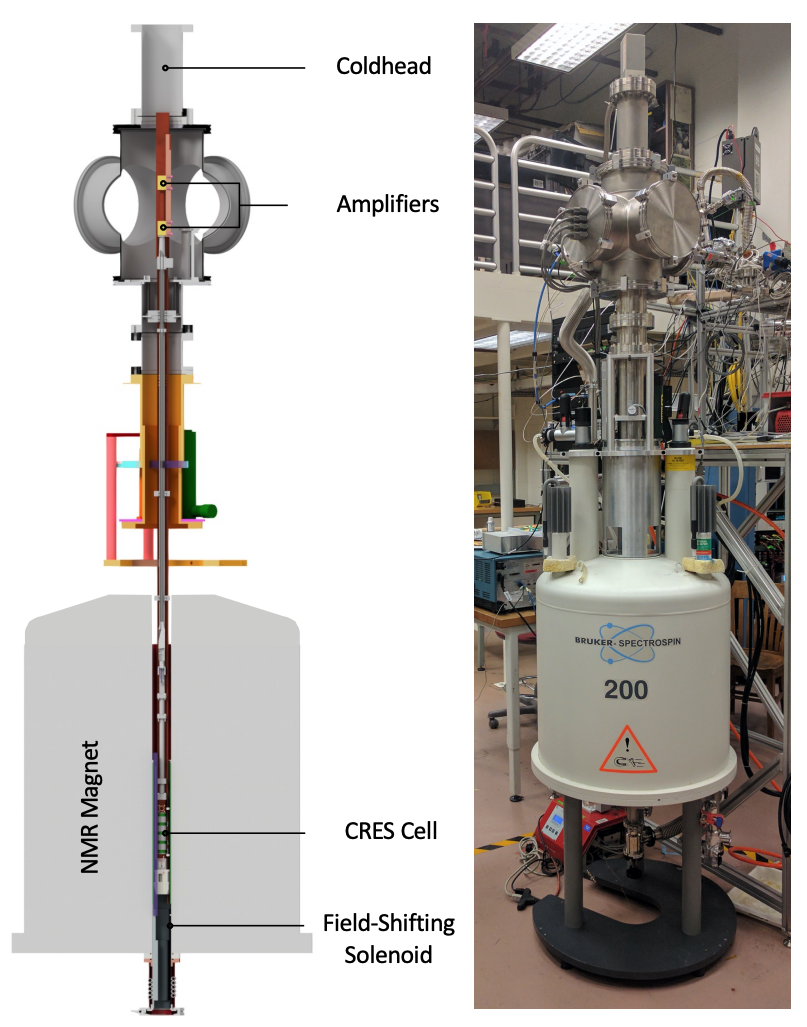
\includegraphics[width=0.55\textwidth]{figs/Chapter-3/phaseII_system.png}
    \caption{\label{fig:chap3-phase2-apparatus} The Phase II CRES apparatus used to perform the first measurement of the tritium beta-decay spectrum using CRES.}
\end{figure}

\subsubsection*{Magnet and Cryogenics}

The magnetic field for the the Phase II experiment is provided by a nuclear magnetic resonance (NMR) spectroscopy magnet with a central bore diameter of 52~mm (see Figure \ref{fig:chap3-phase2-apparatus}). The magnet produces a background magnetic field with an average value of 0.959~T and a 10~ppm variation across the bore diameter achieved using several shim coils built into the magnet. Using an external NMR field probe the variation of the magnetic field along the vertical axis of the magnet bore was measured to obtain an accurate model of the magnetic field so that the CRES cell could be positioned for optimal magnetic field uniformity.

An external solenoid magnet was installed inside the magnet bore to provide the ability to shift the magnitude of the background magnetic field by values on the order of a few mT. The solenoid has inside diameter of 46~mm and a length of 350~mm, which terminates in a vacuum flange that allows it to be inserted into the NMR magnet bore from the bottom. By shifting the value of the magnetic field by a few mT, the cyclotron frequencies of electrons produced by the 17.8~keV $^{83m}$Kr internal-conversion line can be shifted over a range of frequencies on the order of 100~MHz. This allows one to study the frequency dependent behavior of multiple CRES systematics such as detection efficiency that directly affect the measured shape of the tritium spectrum. 

The inside of the magnet bore diameter was pumped down to a vacuum of less than 10~$\mu$torr using a turbomolecular pump, which allows for cryogenic cooling of the CRES cell and RF system. Cooling power was supplied to the Phase II apparatus using a cryopump with its coldhead mounted above the primary magnet and CRES cell. This arrangement allowed for sufficient cooling power to be delivered to the amplifiers to cool them to a temperature of $\approx 40$~K, while keeping the amplifiers far enough from the magnet so as not to be damaged by the large field strength. Thermal contact between the coldhead, amplifiers, RF system, and CRES cell is achieved using a copper bar that runs the full length of the apparatus. To prevent freeze-out of $^{83m}$Kr on the walls of the CRES cell a separate heater was installed to keep the CRES cell near a temperature of 85~K during the operation of the experiment.

\subsubsection*{CRES Cell}

Located in the most uniform region of the magnetic field is the CRES cell, which is the region of the apparatus where radioactive decays of $^{83m}Kr$ and $T_2$ emit electrons that can be trapped and measured using CRES (see Figure \ref{fig:chap3-cres-cell}).
\begin{figure}[htbp]
    \centering
    \includegraphics*[width=0.65\textwidth]{figs/Chapter-3/apparatus.pdf}
    \caption{\label{fig:chap3-cres-cell} Diagram of the CRES cell portion of the Phase II apparatus.}
\end{figure}
The CRES cell is manufactured from a segment of cylindrical waveguide designed to operate at K-band frequencies near 26~GHz. The diameter of the waveguide determines which resonant modes of the waveguide will couple to the electron and transmit its radiation to the amplifiers. For Phase II a waveguide diameter of 1~cm was selected, which allows electrons to couple to the $\mathrm{TE}_{11}$ and $\mathrm{TM}_{01}$ cylindrical waveguide modes. To reduce complexity in modeling and analyzing the CRES data, it is ideal to select a diameter that prevents electrons from coupling to higher-order waveguide modes beyond the fundamental TE and TM modes. 

Around the exterior of the cylindrical waveguide are several magnetic coils used to produce magnetic traps inside the CRES cell volume. Without a magnetic trap electrons produced from decays inside the CRES cell quickly impact the cell wall, which prevents a measurement of their cyclotron frequency using CRES. Each coil along the length of the waveguide produces a separate trap that is approximately harmonic in shape. By independently controlling the currents provided to each coil the traps could be configured to have equal values of the magnetic field at the trap bottom despite a variable background magnetic field from the NMR magnet. 

Two primary magnetic trap configurations were used during the Phase II experiment. The first was a shallow trap configuration used primarily for it's high energy resolution to study systematics using $^{83m}$Kr decays, and the second was a deeper trap that could trap a higher percentage of pitch angles. The trade-off with this trap is that the higher trapping efficiency comes at the cost of lower energy resolution due to the greater variation in pitch angle. The deep trap was the trap used to measure the tritium beta-decay spectrum in Phase II.

The source gases were delivered into the CRES cell through a gas port located near the top end of the cylindrical waveguide. To prevent the gases from escaping the cell, vacuum tight RF transparent windows are needed to contain the tritium and krypton source gas across a 1~atm pressure differential, while still transmitting the cyclotron radiation without distortion. The crystalline material, $\mathrm{CaF}_2$, which has a thermal expansion coefficient similar to that of copper, was used for this purpose in the CRES cell. Two windows, each 2.4~mm thick, were used to seal off the ends of the CRES cell. The thickness of 2.4~mm corresponds to half of a cyclotron wavelength when one accounts for the permittivity of $\mathrm{CaF}_2$.

\subsubsection*{RF System}

The RF system in the Phase II apparatus transferred the cyclotron radiation from the CRES cell to the receiver chain. The receiver chain performs the down-conversion and digitization required to obtain signals that can be analyzed to determine the cyclotron frequencies of electrons in the CRES cell (see Figure \ref{fig:chap3-phase2-rf-chain}).
\begin{figure}[htbp]
    \centering
    \includegraphics*[width=0.95\textwidth]{figs/Chapter-3/230620_phase2_rf_chain.png}
    \caption{\label{fig:chap3-phase2-rf-chain} RF system diagram for the Phase II apparatus.}
\end{figure}

Below the CRES cell, at the bottom of the Phase II apparatus, is a tickler port and waveguide terminator. The tickler port is used to inject signals into the CRES cell and RF system for testing and calibration purposes. The waveguide terminator is designed to absorb cyclotron radiation emitted by electrons that transmits out of the bottom of the CRES cell. This lowers the total power received from electrons in the CRES cell, since all the energy radiated downwards is absorbed into the terminator. Earlier iterations of the Phase II apparatus used an RF short in this location that reflected this power up towards the amplifiers, however, interference between the upward traveling and reflected radiation led to a disappearance in the signal carrier that made reconstruction impossible.

Radiation traveling upward passes through the $\mathrm{CaF}_2$ window passes through a $\lambda/4$ plate, which transforms the circularly polarized cyclotron radiation into linear polarization. The linearly polarized fields next travel through a segment of circular waveguide that transitions into a long segment of WR-42 waveguide that carries the fields out of the high magnetic field region. A thermal break segment is included, which consists of a a segment of gold-plated stainless steel WR-42 waveguide, to help thermally isolate the relatively warm CRES cell from the colder amplifiers. The radiation then passes through a cryogenic circular, which prevents signals reflected from the amplifiers from interfering with the CRES cell before a WR-42 to WR-28 transition connects the waveguide to the first of the cyrogenic amplifiers. The radiation passes through two cyrogenic amplifiers before being coupled to a coaxial termination at the top of the Phase II apparatus.

The coaxial cable transfers the cyclotron radiation signals to a high-frequency mixing stage that performs an analog frequency down-conversion using a 24.5~GHz LO. Two forms of digitization can be used at this stage to readout the CRES data. One is a real-time spectrum analyzer that digitizes the CRES signal data in time-domain and computes the frequency spectrum in real-time, which allows for direct visualization of CRES signal spectrograms as the experiment is running. The real-time spectrum analyzer is most useful for taking small amount of streamed data for debugging and analysis of the system. The other method, which was used to collect the majority of the CRES data in Phase II, is a ROACH-2 FPGA and digitizer system. The ROACH system consists of a fast ADC that samples the CRES signal data at 3.2~GSps. Internal digital down-conversion stages implemented in the FPGA perform a mixing operation that reduces the bandwidth of the CRES signals to 100~MHz. The FPGA implements a 8192 sample FFT and packetizes time and frequency domain records in parallel. The packetized data is then transferred from the ROACH to be analyzed by the data-processing pipeline.

\subsection{CRES Track and Event Reconstruction}

\subsubsection*{Time-Frequency Spectrogram}

The online data-processing is intended to identify interesting data that could contain CRES signals using a software real-time triggering algorithm. Interesting segments of data identified by this algorithm are collected into files that are transferred to a server for offline processing and analysis. The data files contain a continuous series of time-domain samples, broken into a set of records, which are 4096 samples long. The time-series is made up of 8-bit IQ samples acquired at 100~MHz. 

Each time-series record is accompanied by an associated frequency spectrum consisting of 4096 frequency bins approximately 24.4~kHz wide, which is represented as a power spectral density. The individual frequency spectra can be organized temporally to create a time-frequency spectrogram that represents the evolution of the cyclotron frequency spectrum over the course of the CRES event (see Figure \ref{fig:chap3-tritium-event0-spectrogram}). 
\begin{figure}[htbp]
    \centering
    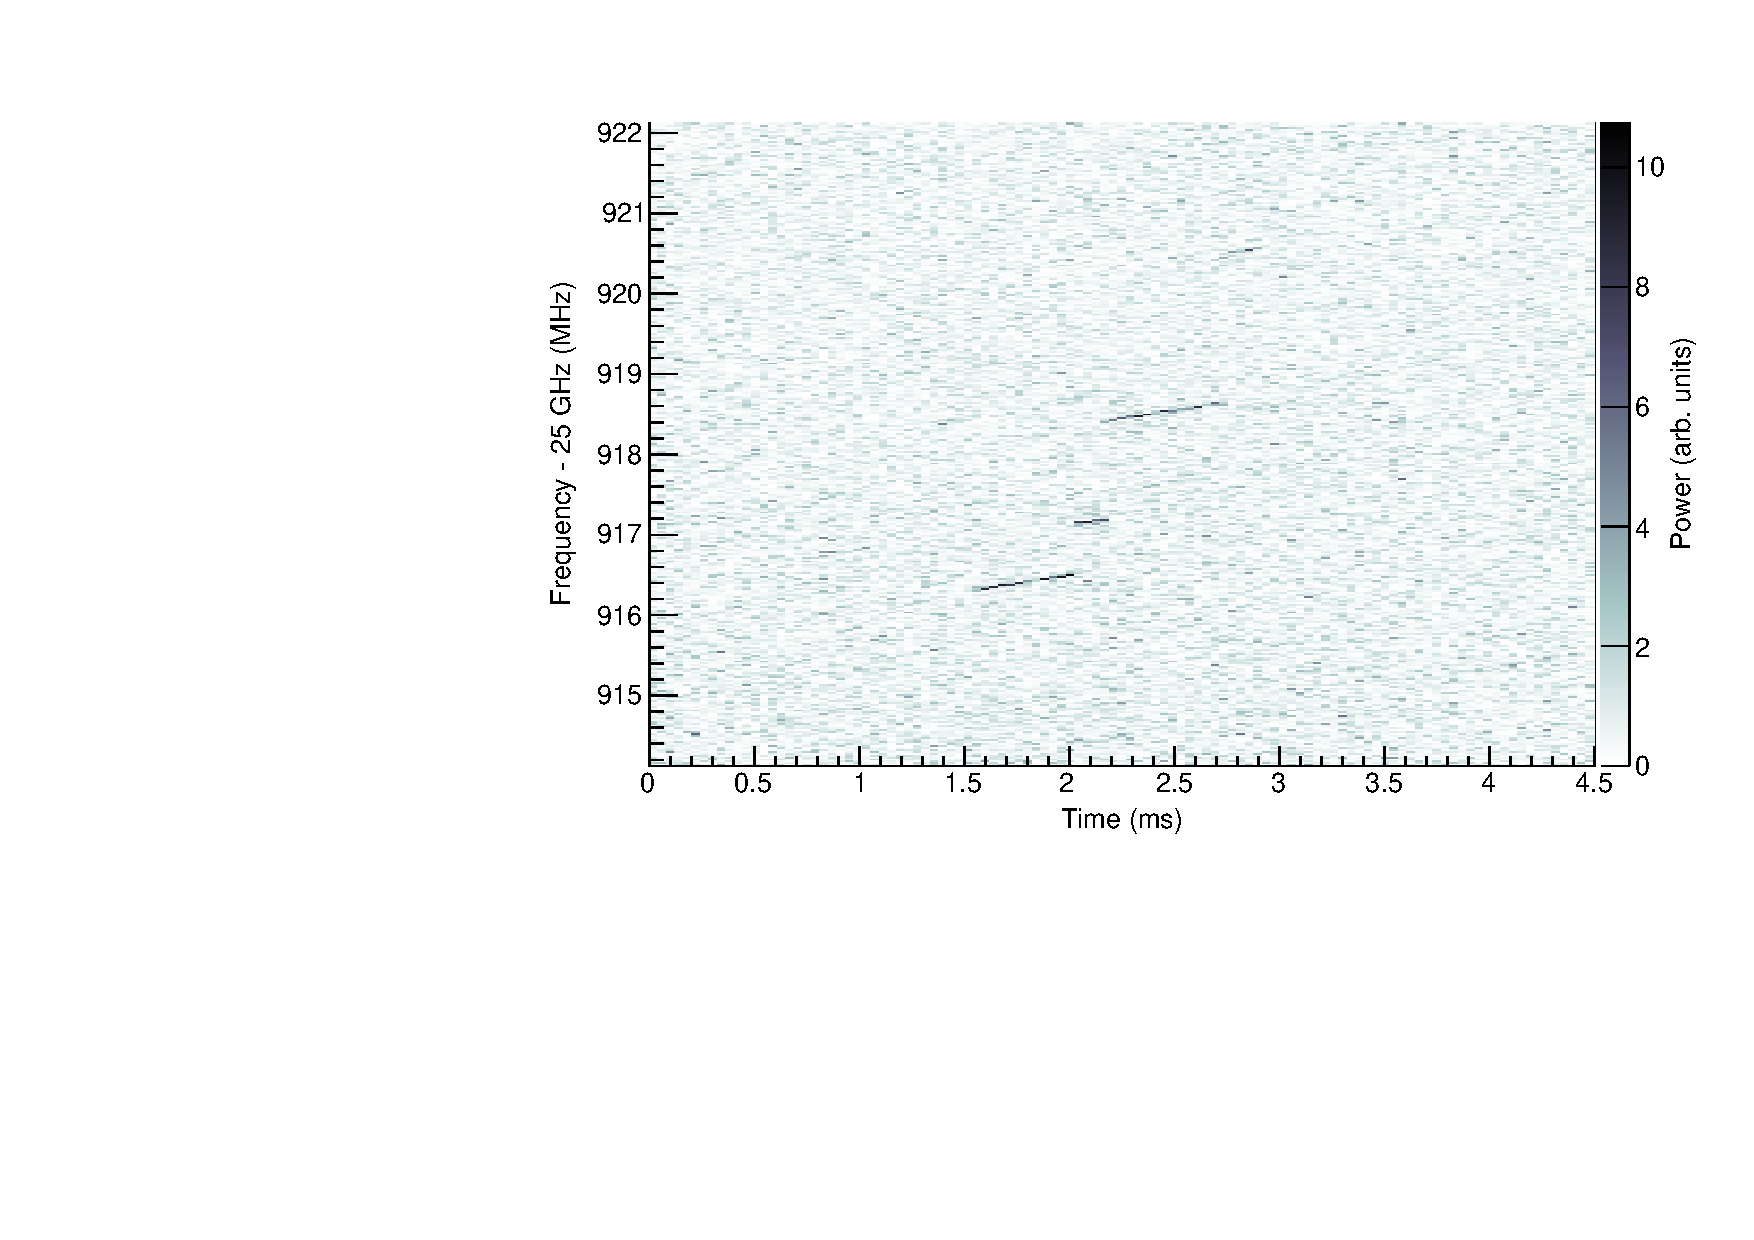
\includegraphics[width=0.7\textwidth]{figs/Chapter-3/T2_Event0.pdf}
    \caption{The time-frequency spectrogram of a tritium CRES event in the Phase II apparatus.}
    \label{fig:chap3-tritium-event0-spectrogram}
\end{figure}
The time-frequency spectrogram is represented as a two-dimensional image where the color of each pixel is proportional to the power spectral density. Each vertical slice of pixels in the image represents a frequency spectrum, therefore, each horizontal bin represents the data obtained over a duration of $4096\times 0.01$ $\mathrm{MHz}^{-1}=40.96$ $\mu$sec. 

\subsubsection*{CRES Event Data Features}

Phenomenologically, a CRES signal appears as a sinusoidal signal whose frequency slow increases ("chirps") over time. Axial motion of the electron in the trap leads to the formation of frequency sidebands that surround the more powerful carrier frequency, due to doppler modulation of the electron's frequency as it bounces between the walls of the magnetic trap. The critical piece of information that must be extracted from the track and event reconstruction procedure is the carrier frequency, since it is this frequency that gives the cyclotron frequency and thus the kinetic energy. While axial motion from non-$90^\circ$ pitch angles does change the average magnetic field experienced by an electron and, therefore, changes the cyclotron frequency. We were not able to resolve sidebands in Phase II, so a correction for the effect of the pitch angle on the cyclotron frequency was not possible. 

In the time-frequency spectrogram representation the chriping carrier frequency appears as a linear track of high-power frequency bins (see Figure \ref{fig:chap3-tritium-event0-spectrogram}). The vertical slope of the tracks is caused by the emission of energy from from the electron in the form of cyclotron radiation, therefore, the size of the slope parameter is directly proportional to the Larmor power. The continuous track is periodically interrupted by random jumps to higher frequency and lower energy caused by random inelastic collisions with background gas molecules. The length of a track is an exponentially distributed variable whose mean value is inversely proportional to the gas density. The size of the frequency discontinuities is directly proportional to the energies of the rotational and vibrational states of background gas species such as $CO_2$. 

A CRES event refers to the collection of tracks produced by a trapped electron until it inevitably scatters into a pitch angle that can no longer be trapped. The goal of track and event reconstruction is to first identify the set of tracks present in a time-frequency spectrogram that represents a segment of data acquired in the Phase II apparatus. These tracks must then be clustered into events from which we can determine the first track produced by the electron and thus estimate it's starting cyclotron frequency and kinetic energy. 

\subsubsection*{Track Reconstruction}

The first step in this process is the identification of tracks in the time-frequency spectrogram, which is essentially an image processing feature identification task. The first step in the track finding procedure is to normalize the power spectral density based on the average noise power to obtain the time-frequency spectrogram in the form of normalized, unitless power. Next a power threshold is applied to the normalized spectrogram where only bins that have a signal-to-noise ratio greater than five are selected to build tracks. In this case signal-to-noise ratio is defined as the ratio between the normalized, unitless power of a bin divided by the average normalized power across the full frequency spectrum.

\begin{figure}[htbp]
    \centering
    \includegraphics*[width=0.7\textwidth]{figs/Chapter-3/230621_t_event_zero_sparse_spectrogram_zoom.pdf}
    \caption{\label{fig:chap3-sparse-spectrogram} The sparse spectrogram obtained by placing a power cut on the raw spectrogram shown in Figure \ref{fig:chap3-tritium-event0-spectrogram}.}
\end{figure}

The spectrogram produced by this power cut, termed the sparse spectrogram, consists only of a sparse collection of high-power frequency bins that could be part of a CRES signal track (see Figure \ref{fig:chap3-sparse-spectrogram}). In this form is it much easier to identify tracks "by eye", however, for the Phase II analysis Project 8 developed it's own custom-made track finding algorithm, called the sequential track finder (STF). 

The STF algorithm process the sparse spectrogram in sequential fashion, processing each time-slice one-by-one until the end of the spectrogram is reached. Tracks are found by searching for points in the sparse spectrogram that appear to fall on a straight line. Multiple configurable parameters are built into the STF algorithm that allow the user to tune the criteria for adding a point to an existing track or creating a brand new track. These include parameters such as maximum time and frequency differences between subsequent points in a track as well as minimum SNR values for the start and endpoints of the track. Additionally, tracks are required to have a minimum length and slope to be considered potential CRES tracks rather than random noise fluctuations. 

The resulting output of the STF is a collection of track objects that consist of all of the points that make up the track and their properties. The final step in track reconstruction is to calculate the track properties and apply final cuts to reject the majority of false tracks found by the STF. This involves the fitting of a line to the collection of track points as well as the total and average power of the track obtained by computing the sum and mean of the points powers. The starting frequency of the track is determined by calculating the time coordinate that  intersects with the linear fit. A cut is the performed to remove all tracks that do not have a specified average power over their duration, which helps to remove the majority of noise fluctuations that have passed all previous cuts up to this point.

\subsubsection*{Event Reconstruction}

The final step is event reconstruction where the identified tracks are grouped into events that contain all tracks likely caused by the same electron. This procedure simply attempts to match tracks head to tail by checking if the start and end times of a pair of tracks falls withing a certain tolerance. This tolerance is an additional configurable parameter that can be tuned to an optimal value using monte carlo simulations of events in the Phase II apparatus.

After the event building procedure has completed there is still a small likelihood that false tracks have made it through to this stage in the reconstruction. Typically, cuts at the track level are able to remove 95\% of the false tracks identified by the STF, which leads to a significant number of false tracks at the event building stage. However, the additional event-level information makes it possible to reject events that contain these false tracks with a high degree of confidence. 

Two event level features are associated with events caused by real electrons --- the duration of the first track as well as the number of tracks in the event. Real electrons tend to have event structures with longer first tracks and a higher number of total tracks. Based on the values of these two criteria, a minimum threshold on the average power in the first track was configured to reject false events. The average power in the first track was chosen due to the critical nature of the starting frequency of the first track in an event to the krypton and tritium spectrum analyses.

\subsection{Results from Phase II}

The primary result from Phase II is the first-ever measurement of the tritium beta-decay spectrum using CRES, which lead to the first neutrino mass limit using the CRES technique. However, Phase II also included a significant $^{83m}\rm{Kr}$ measurement campaign to understand important systematics relevant to the tritium spectrum measurement, but also to understanding the fundamentals of the CRES technique itself. This required high-resolution measurements of the $^{83m}\rm{Kr}$ internal-conversion spectrum, which is an interesting science result in its own right.

The results from Phase II represents a significant effort from the entire Project 8 collaboration over several years. Because the focus of my contributions to Project 8 is directed towards the research and development efforts for the Phase III experiments, the goal in this section is not to provide a detailed description of the the analyses that lead to the Phase II results. Rather, I will provide brief descriptions of a few plots representative of the main results from Phase II and direct the interested reader to the relevant Phase II papers.  

\subsubsection*{Measurements with Krypton}

Measurements with krypton were a key calibration tool for Phase II of the experiment and will most likely continue to be useful in future Phases of Project 8. In the context of Project 8 krypton measurements refers to CRES measurements of the internal-conversion spectrum of the metastable state of krypton-83, $^{83m}\rm{Kr}$, produced by electron capture decays of $^{83}\rm{Rb}$. A supply of $^{83}\rm{Rb}$ was built into the Phase II apparatus gas system that supplied the CRES cell with $^{83m}\rm{Kr}$ via emanation.

The $^{83m}\rm{Kr}$ internal-conversion spectrum consists of several lines based on the orbital of the electron ejected during the decay. The conversion lines useful to Project 8 are those that emit electrons with kinetic energies that fall inside the detectable frequency bandwidth of the Phase II apparatus. These are the K; L2 and L3; M2 and M3; and N2 and N3 lines with kinetic energies of 17.8~keV, $\approx 30.4$~keV, $\approx 31.9$~keV, and $\approx 32.1$~keV, respectively. The different energies of the lines allow us to test the linearity of the relationship between kinetic energy and frequency across the range of frequencies covered by the continuous tritium spectrum.

\begin{figure}[htbp]
    \centering
    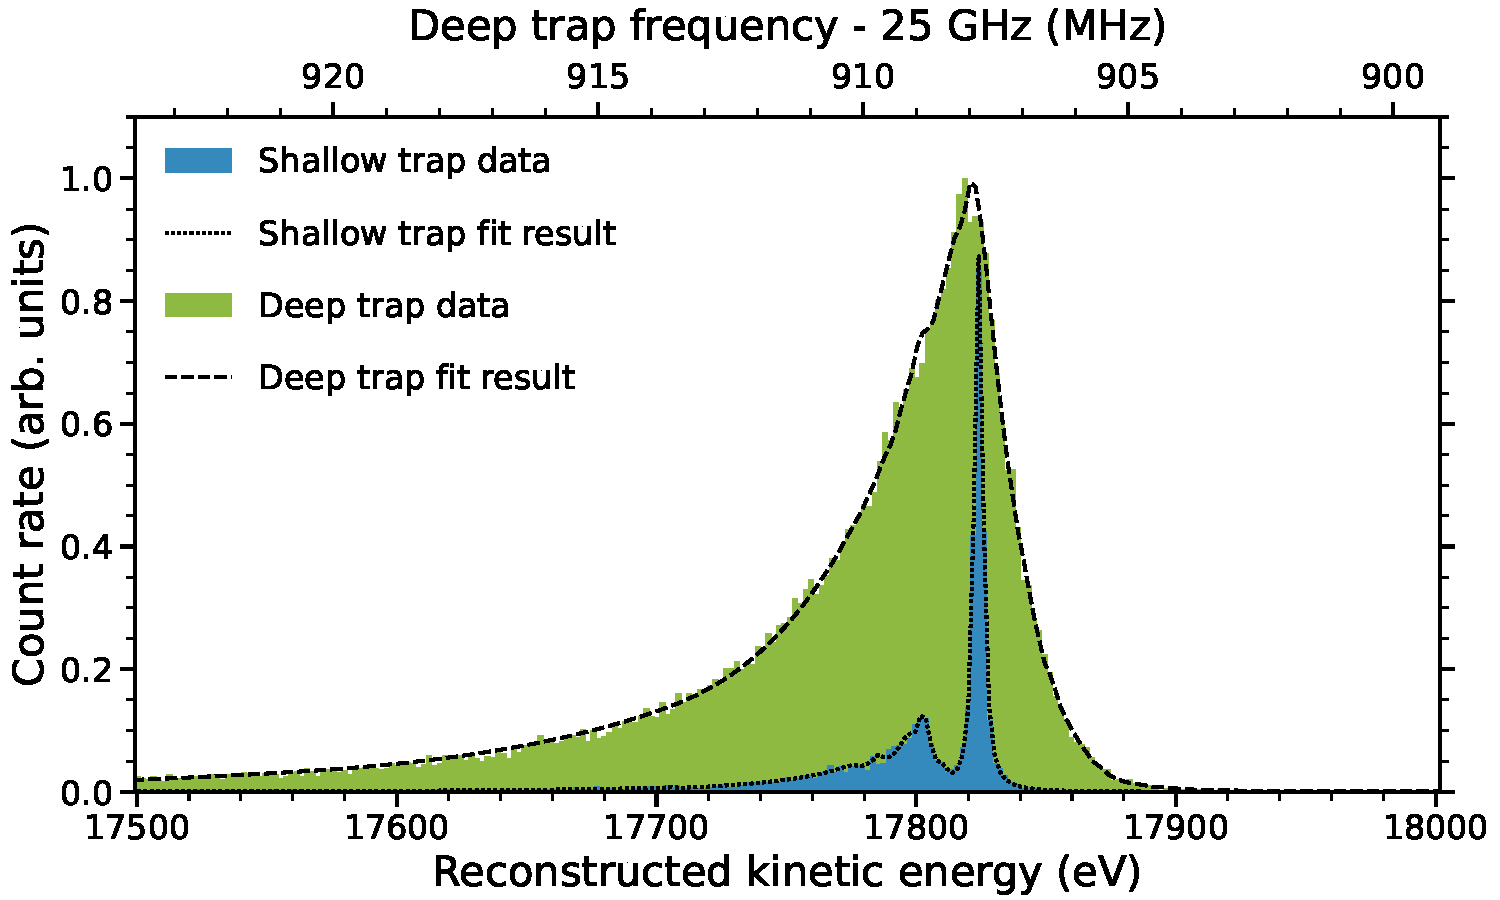
\includegraphics[width=0.7\textwidth]{figs/Chapter-3/kr_fit.pdf}
    \caption{Fits to the measured 17.8-keV $^{83m}\rm{Kr}$ conversion line using the deep and shallow trap configurations. }
    \label{fig:chap3-krypton-spec-fit}
\end{figure}

By measuring the shape of the krypton spectrum we can characterize the effects of numerous detector related effects relevant to the tritium analysis. Specific examples include the variation in the magnetic field as a function of the radial position of the electron, variation in the magnetic field caused by the trap shape, variation in the average magnetic field for electron of different pitch angles, the effect of missing tracks due to scattering, among others. These spectrum shape measurements focused on the 17.8-keV krypton line and utilized different trap geometries based on the particular goal of the dataset (see Figure \ref{fig:chap3-krypton-spec-fit}).

Krypton measurements with a shallow trap allow for high energy resolution, since variation in frequency due to pitch angle differences is sharply reduced in the shallow trap configuration. With this trap the main 17.8-keV peak of the conversion spectrum is clearly visible along with additional satellite peaks at lower energy, which correspond to the shakeup/shakeoff spectrum of the decay. The high accuracy of the fit demonstrates a high degree of understanding of the CRES systematics.

\begin{figure}[htbp]
    \centering
    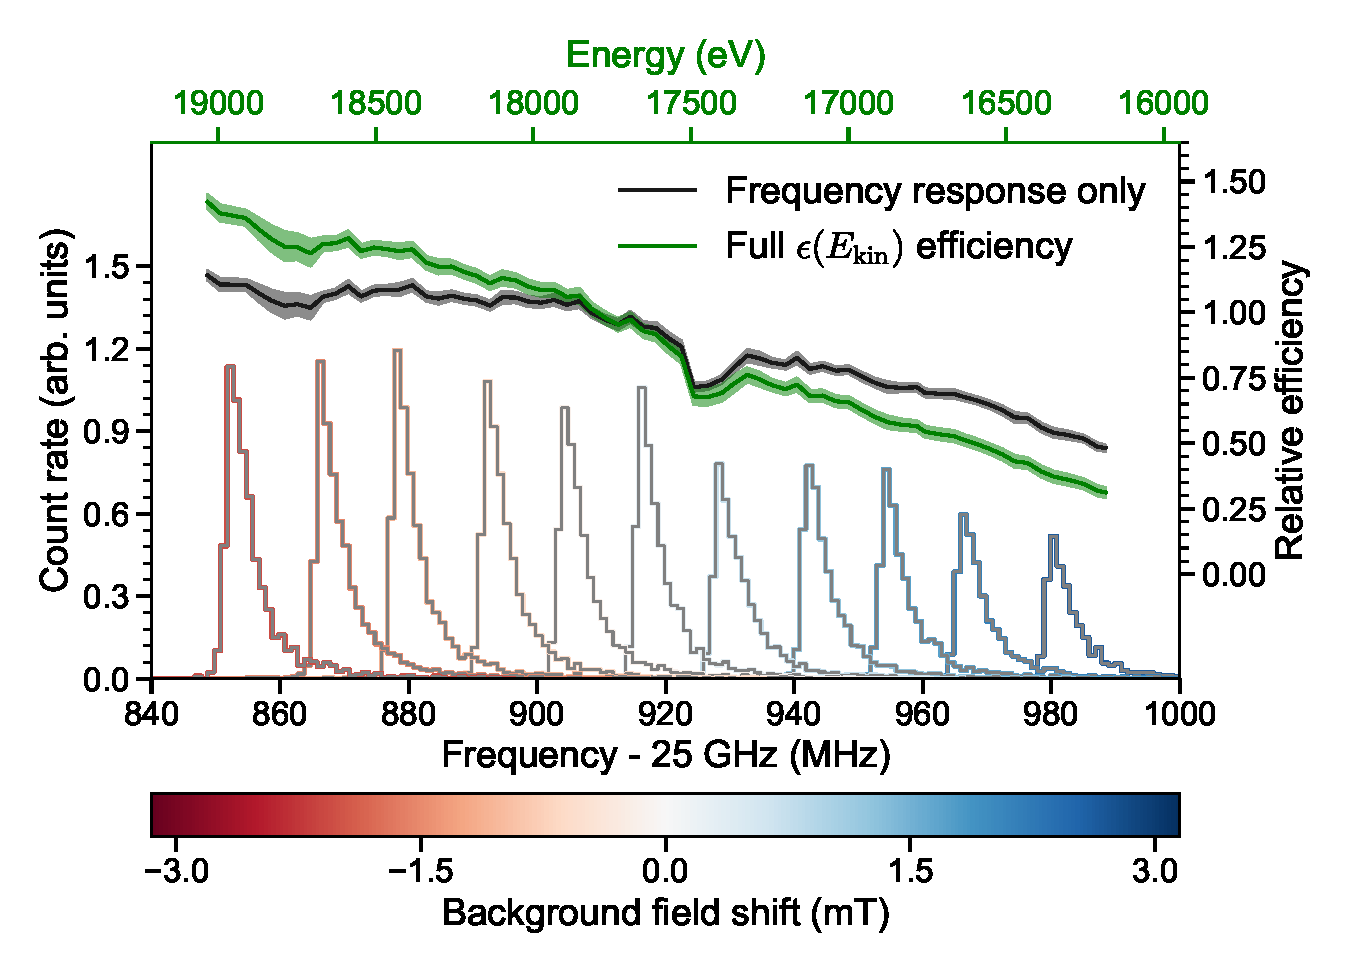
\includegraphics[width=0.7\textwidth]{figs/Chapter-3/fss_for_prl_plot.pdf}
    \caption{Measurements of the 17.8-keV $^{83m}\rm{Kr}$ line using the deep trap configuration for different values of the magnetic field from the field shifting solenoid.}
    \label{fig:chap3-fss-plot}
\end{figure}

The broadening of the krypton spectrum seen for the deeper track is due to the higher range of electron pitch angles that can be trapped. Furthermore, with a deeper trap there is a larger parameter space of electron that could be produced with pitch angles that are trappable but not not visible in the time-frequency spectrogram. These electrons live in the trap can can scatter multiple times before randomly scattering to a pitch angle that is now visible. This causes us to miss one to several of the electron's tracks earlier in the event, which leads us to mis-reconstruct the true starting frequency of an event. By measuring the krypton spectrum shape in the same deep trap used to detect tritium events we can characterize the affect that this has on the spectrum shape to mitigate it's impact on the tritium measurements.

An additional systematic characterized with krypton is the calibration of the detection efficiency of the Phase II apparatus as a function of frequency. Variations in the detection efficiency as a function of frequency directly changes the measured shape of the continuous tritium spectrum, which can lead to errors in the neutrino mass estimate if not modeled appropriately. Using the field shifting solenoid the cyclotron frequency of the krypton 17.83~keV line was shifted across the full frequency range of the tritium spectrum data (see Figure \ref{fig:chap3-fss-plot}). Variations in the deep trap krypton spectrum shape can be used to infer the detection efficiency as a function of frequency and correct for this affect in the tritium measurements.

\subsubsection*{Tritium Spectrum and Neutrino Mass Results}

The tritium measurement campaign resulted in the collection of 82 days of detector live time during which 3770 total tritium events were detected. The track and event reconstruction analysis extracted the starting frequencies of these tritium events, which were used to build a frequency spectrum of tritium beta-decays. The resulting frequency spectrum was then converted to an energy spectrum using the information gleaned from the krypton measurement campaign to obtain the tritium beta-decay spectrum (see Figure \ref{fig:chap3-final-tritium-fit}).
\begin{figure}
    \centering
    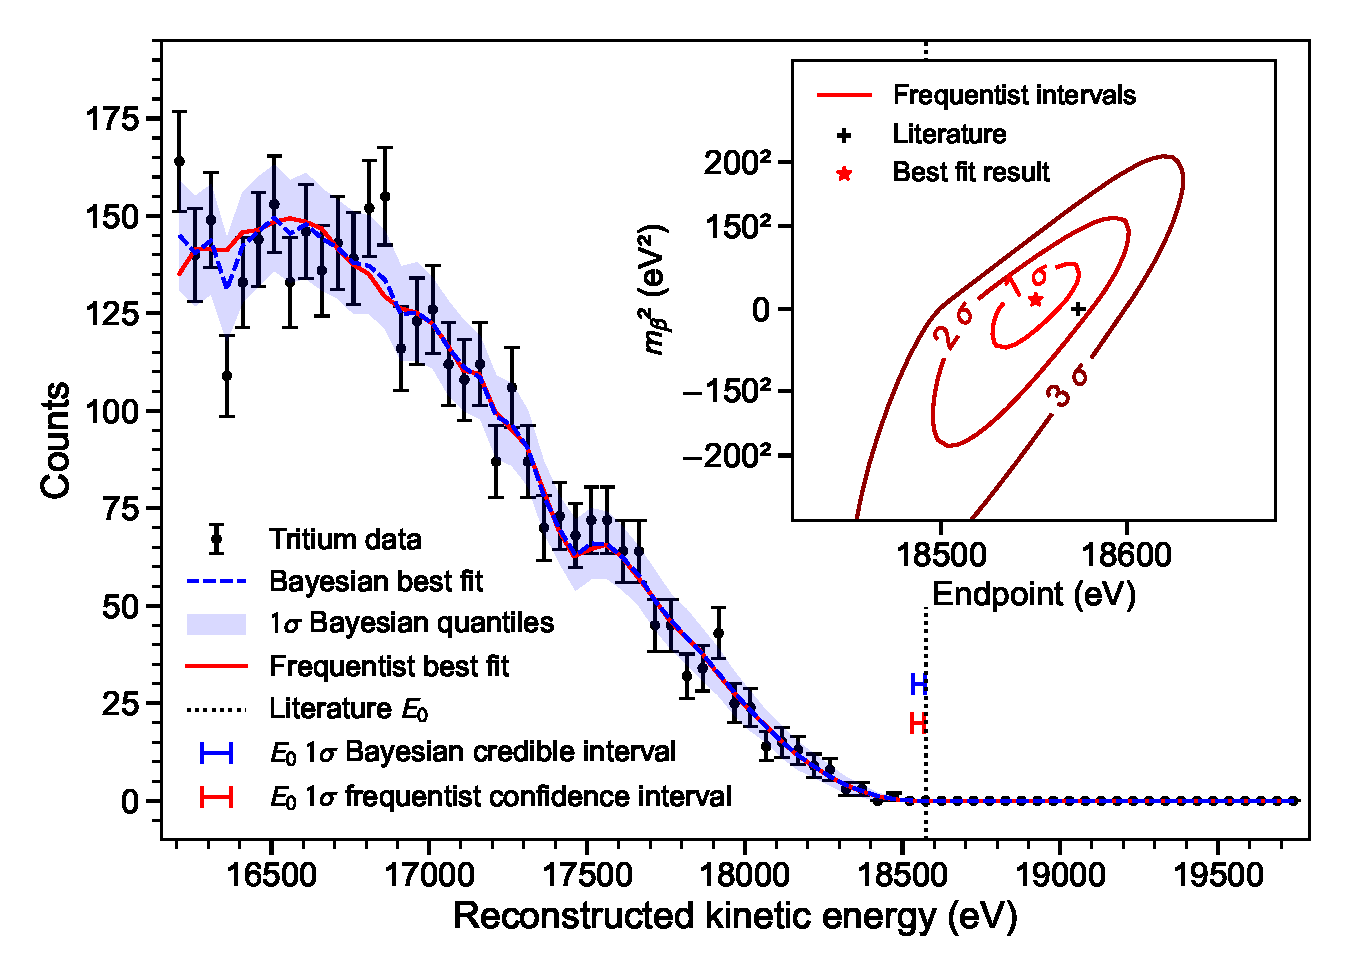
\includegraphics[width=0.7\textwidth]{figs/Chapter-3/12-03-22A_final_E0_real_data_phase_II_tritium_fit_1d.pdf}
    \caption{The measured tritium spectrum from Phase II with Bayesian and frequentist fits.}
    \label{fig:chap3-final-tritium-fit}
\end{figure}

CRES is inherently a very low background technique with the dominant source of noise being random RF fluctuations. Monte carlo simulations backed up by measurements of the RF noise background were used to set track and event characteristic cuts to guarantee that zero false events would occur over the duration of the experiment with 90\% confidence. Notably, the measured spectrum has zero events beyond the tritium spectrum endpoint, which allows us to constrain the background rate in the Phase II apparatus to less than $3\times10^{-10}$~counts/ev/s. Achieving a low background is critical for future neutrino mass experiments that seek to measure the neutrino mass with less than 100~meV sensitivity.

Bayesian and frequentist based fits to the measured tritium spectrum, incorporating information gained about CRES systematics from the krypton measurements, were performed to extract upper limits on the tritium beta-decay spectrum endpoint as well as the neutrino mass. The estimated spectrum endpoints are $18553^{+18}_{-19}$~eV for the Bayesian analysis and $18548^{+19}_{-19}$~eV for the frequentist analysis. The quoted uncertainties are 1-$\sigma$, and both results are within 2-$\sigma$ of the literature endpoint value of 15574~eV. The estimated neutrino mass for both results is consistent with $m_\beta^2=0$. The 90\% confidence upper limits for the Bayesian analysis is $m_\beta < 155$~$\rm{eV}/\rm{c}^2$ and $m_\beta < 152$~$\rm{eV}/\rm{c}$ for the frequentist analysis.

Though the neutrino mass results from Phase II are not competitive with KATRIN it is a promising first step towards the development of more precise neutrino mass measurements using CRES. The low background and demonstrated high resolution with krypton measurements are promising features of the technique that were able to be demonstrated with the Phase II apparatus. As new technologies are developed to enable CRES measurements in larger volume, many of the lessons learned from Phase II will continue to influence the operation and design of the detectors.

\section{Phase III R\&D: Antenna Array CRES}
\label{sec:chap3-phaseIII-antenna-arrays}

The goal of Phase III in the Project 8 experimental program is to develop the technologies and expertise required to build an experiment that uses CRES to measure the neutrino mass with a target sensitivity of 40~meV. One of the key technologies is a method for performing high resolution CRES measurements in a large volume, which allows one to observe a sufficient quantity of tritium to measure the low-activity endpoint region of the tritium spectrum. 

\subsection{The Basic Approach}

One possible approach, suggested in the original CRES publication, is to use many antennas to surround a volume of tritium gas in a magnetic field (see Figure \ref{fig:chap3-antenna-concept-cartoon}). When a decay occurs the electron will begin to emit cyclotron radiation that can be collected by the array and used to perform CRES.
\begin{figure}[htbp]
    \centering
    \includegraphics*[width=0.6\textwidth]{figs/Chapter-3/230614_antenna_cartoon.png}
    \caption{\label{fig:chap3-antenna-concept-cartoon} A cartoon illustration of the basics of the antenna array CRES technique.}
\end{figure}
Each antenna in the array collects only a small fraction of the electron's signal power, which is less than 1~fW for a 18.6~keV kinetic energy electron in a 1~T magnetic field. Scaling to large volumes with the antenna array approach is accomplished by increasing the number of antennas in the array, which increases the volume under observation proportionally, so that a sufficient population of tritium atoms can be observed to measure the tritium spectrum endpoint shape. 

Several features of the antenna array approach make it an attractive candidate technology for a large volume experiment. One example is the accurate position reconstruction made possible by the multichannel nature of the array. Using techniques like digital beamforming it is possible to estimate the radial and azimuthal positions of the electron in the magnetic trap with a precision significantly less than the size of the cyclotron wavelength. This capability allows one to perform event-by-event estimations of the magnetic field experienced by an electron, which is crucial to achieving high energy resolution with the CRES technique.

The easy availability of position information with the antennas array approach is potentially a unique advantage that provides significant flexibility in the magnetic field uniformity requirements compared to other proposed approaches to large volume CRES (see Chapter \ref{chap:cavity}). Spatial discrimination using digital beamforming leads to pileup reduction, which helps to reduce the potential of background events caused by missing tracks or by incorrectly clustering a group of tracks into an event. Limits on the background rate for a neutrino mass measurement with 40~meV sensitivity are stringent and the total activity of the tritium source for such an experiment is gigantic relative to the activity near the endpoint. Thus, pileup discrimination could be an important tool for a large scale CRES experiment.

Another beneficial quality of the antenna array approach is that the volume of the experiment can be scaled independent of frequency by simply adding more antennas to the array (see Figure \ref{fig:chap3-phaseiv-antenna}). Resonant cavities, the proposed alternative large volume CRES technology, are ideally operated in magnetic fields that cause electrons to move with cyclotron frequencies near the fundamental cavity resonance, to avoid complex coupling of the electron to many cavity modes simultaneously. This leads to a coupling between the cavity volume and the magnetic field magnitude, which forces one to lower the magnetic field in order to increase the experiment scale. Whereas, for antenna arrays, in principle there is no physical limitation on the size of the antenna array that can be used at a particular magnetic field. However, the nature of scaling an antenna array based experiment leads to rapidly increasing cost and complexity due to the large number of antennas, amplifiers, and data streams that require substantial computer processing power to effectively analyze.

\subsection{The FSCD: Free-space CRES Demonstrator}

The complex collection of new experimental techniques and methods that come together in the antenna array CRES technique require the construction of a small scale demonstration experiment designed to develop an understanding of the principles of antenna array CRES measurements and the relevant systematics. Without operating such an experiment it is not possible to develop a design for a large scale CRES experiment with sufficient confidence that the experiment is capable of measuring the shape of the tritium spectrum endpoint to the degree of accuracy required for 40~meV sensitivity to the neutrino mass. Therefore, Phase III of the Project 8 experimental program is primarily focused on the development and operation of demonstrator experiments to inform the design of the final Phase IV experiment.

Specifically for antenna array CRES, the associated demonstrator experiment in Phase III is called the Free-space CRES Demonstrator or FSCD. The goals of the FSCD include not only the development of antenna array CRES itself, but is also a capable neutrino mass measurement experiment in it's own right, with a target neutrino mass sensitivity of a few eV using a molecular tritium source.  

\subsubsection*{Magnetic Field}

The background magnetic field for the FSCD experiment is provided by a hospital-grade MRI magnet (see Figure \ref{fig:chap3-mri-magnet}). The magnet produces a magnetic field of approximately 0.958~T, which corresponds to a tritium spectrum endpoint frequency of approximately 25.86~GHz. 
\begin{figure}[htbp]
    \centering
    \includegraphics*[width=0.5\textwidth]{figs/Chapter-3/230614_mri_magnet.png}
    \caption{\label{fig:chap3-mri-magnet} An image of the MRI magnet installed in the Project 8 laboratory at the University of Washington, Seattle.}
\end{figure}
The magnet is installed in the Project 8 laboratory located at the University of Washington, Seattle, and is shimmed to produce a uniform magnetic field with variations on the ppm scale. Measurements of the magnetic field non-uniformities were performed using a NMR probe and rotational gantry to capture measurements of the magnetic field around an elliptical surface in the center of the MRI magnet. During the operation of the FSCD an array of Hall or NMR magnetometers could be used to periodical measure the magnetic field in order to quantify its time stability.

Inside the main magnetic field of the MRI magnet are additional magnets that provide the capability to shift the value of the background magnetic field as well as the magnets that produce the magnetic trap. Shifting the background value of the magnetic field on a scale of $O(\mu T)$ allows one to control the cyclotron frequencies of electrons with a fixed kinetic energy, which is key to effectively calibrating the FSCD. The preferred calibration method for the FSCD is a mono-energetic electron gun that can inject electrons into the magnetic trap with a known kinetic energy. In combination with the field shifting magnet one can vary the cyclotron frequencies of the electrons to measure the response of the antenna array as a function of the radiation frequency and electron position. This procedure not only characterizes the response of the antenna array but also provides further information on magnetic field uniformity, which important to achieving optimal energy resolution.

Several additional magnetic coils will need to included inside the MRI magnet to produce the magnetic trap. The ideal trap shape for CRES is the perfect magnetic box, which has a flat bottom and step function walls. Any variation in the average magnetic field experienced by an electron leads to changes in the cyclotron frequency that can make determining the true starting kinetic energy more difficult. This includes changes in the magnetic field caused by the walls of the magnetic trap as well as radial magnetic field variations. The perfect box trap is completely uniform and has infinitely steep walls that cause no change in the electron's cyclotron frequency as it is reflected from the trap wall, however, such a trap cannot be made from any combination of magnetic coils since it violates Maxwell's equations. The goal of magnetic trap design is to identify the configuration of coils that produces a trap that approximates the perfect box trap as closely as possible.

\subsubsection*{Antenna Array}

The canonical antenna array design for a CRES experiment is a uniform cylindrical array of antennas that surrounds the magnetic trap volume. Since the FSCD is a demonstrator experiment, the antenna array design is the simplest form of the uniform cylindrical array, which is a single circular ring of antennas with a diameter of 20~cm (see Figure \ref{fig:chap3-fscd-render}).
\begin{figure}[htbp]
    \centering
    \begin{subfigure}{0.5\textwidth}
        \includegraphics*[width=\textwidth]{figs/Chapter-3/230614_fscd_render.png}
        \caption{}
    \end{subfigure}
    \hfill
    \begin{subfigure}{0.4\textwidth}
        \includegraphics*[width=\textwidth]{figs/Chapter-3/230614_5slot_model.png}
        \caption{}
    \end{subfigure}
    \caption{\label{fig:chap3-fscd-render} (a) A model of the FSCD antenna array, magnetic trap, and tritium containment vessel design.(b) A more detailed model of a prototype design for the 5-slot waveguide antenna design.}
\end{figure}
Along this circle are sixty slotted waveguide antennas that fully populate the available space around the array circumference. In order to maximize the power collected from each electron it is optimal to cover as large a fraction of the solid angle around the magnetic trap as possible. 

The distance between antennas around the circumference of the array is proportional to the wavelength of the cyclotron radiation. Therefore, maximizing the solid angle coverage of the array, while minimizing channel count to keep the hardware and data acquisition costs manageable, biases one towards smaller array diameters. Antenna near-field effects limit the minimum diameter of the array for a given antenna design since the radiation from electron's that are too close to the array cannot be detected due to destructive interference caused by path-length differences from the electron to different points on the antenna surface. 

Slotted waveguide antennas are used in the FSCD antenna array due to their high efficiency and low loss, which comes from the lack of dielectric materials in the antenna structure. Coupling to the waveguide can be performed with a coaxial cable connected at the center or on either end of the waveguide. One of the drawbacks of waveguide antennas is the large amount of space required to fit them inside the limited MRI magnet volume. Alternative antenna designs, constructed from microstrip printed circuit boards require significantly less space at the cost of slightly higher energy loss in the antenna structure. 

The FSCD antenna design is a 5~cm long segment of WR-34 waveguide with 5 vertical slots cut into the side. The distance between slots along the length of the waveguide is a half wavelength for optimal power combination between the individual antenna slots. Each slot is offset from the center of the antenna face a small distance in order to most effectively couple the slot to waveguide modes inside the antenna.

The passive power combination achieved by placing 5 slots in a single waveguide is a compromise intended to reduce the cost and complexity of the antenna array system. Each additional channel in the array requires it's own cryogenic amplifier and also increase the required computer power to process the raw data collected by digitizing each channel. Passive summation, achieved by combining antennas into arrays axially, reduces the array channel count at the cost of losses from imperfect passive combination. Imperfect passive combination is caused by effects such as re-radiation of energy from and destructive interference between slots in the waveguide antenna. 

Interference and re-radiation eventually limit the achievable the axial extent of passive power combination. The 5-slot designed developed for the FSCD is optimized to minimize the impact of these losses while achieving the maximum amount of axial coverage with a single ring of antennas. Scaling beyond the volume covered by a single ring of antennas is achieved by stacking additional rings of antennas together to cover a larger trap volume for a higher statistics measurement of the tritium spectrum endpoint region. A likely scenario for the FSCD experiment involves a staged experiment approach, where first a series of measurements is performed using only a single ring of antennas followed by experiments that add additional rings to the FSCD. The goal would be to first understand the principles of antenna array CRES using the simplest possible experiment, before attempting to scale the technique by expanding the antenna array size. 

\subsubsection*{Tritium Source}

While the primary purpose of the FSCD is as a technology demonstrator, it is unlikely for the collaboration to gain the required confidence in the antenna array CRES technique to perform neutrino mass measurements at the 40~meV sensitivity level without an intermediate scale measurement of the neutrino mass using antenna array CRES. Therefore, the FSCD has an additional scientific goal of measuring the neutrino mass with a rough sensitivity goal of a few eV. This level of precision is achievable using a source of molecular tritium with a volume of approximately 1~L at a density comparable to potential Phase IV scenarios.

Unlike previous CRES experiments, where the tritium source could be co-located with the receiving antenna inside a waveguide transmission line, the tritium source in the FSCD is thermally isolated from the antenna array to avoid freeze-out of the tritium molecules. The tiny radiation power emitted by electrons requires a system noise temperature of $\approx 10$~K or less, in order to detect events at a high enough efficiency to reach the neutrino mass sensitivity goals of the experiment. Achieving a system noise of 10~K requires that the antenna array and amplifiers operate at cryogenic, liquid helium temperatures of $\approx 4$~K, which significantly lowers the vapor pressure of molecular tritium. By keeping the molecular tritium isolated in an RF-transparent vessel the tritium gas can be kept at a relatively warmer temperature in the range of 30~K to avoid the accumulation of tritium on the experiment surfaces. 

\subsubsection*{Data Acquisition and Reconstruction}

A fundamental change in the data acquisition system for the FSCD is the shift from single to multi-channel reconstruction. This transition results in a significant increase in the data-generation rate, which is linearly related to the number of independent channels in the array. The larger data volume coincides with an increased demand for computer processing power based on the need for more precise signal reconstruction algorithms driven by the FSCD and Phase IV sensitivity goals. Therefore, the data acquisition system for the FSCD is likely to represent a significantly larger fraction of the experiment cost and complexity than previous CRES experiments.

Each antenna in the array is connected to a cryogenic amplifier and down-converted from the 26~GHz CRES frequency using an IQ-mixer to reduce the size of the analysis window in which the tritium spectrum is measured. Using an LO with a frequency of approximately 25.80~GHz the antenna array signals can be digitized at a rate of 200~MHz, which is sufficient bandwidth to resolve the complete sideband spectrum produced by axial oscillations of electrons in the FSCD magnetic trap. 

Direct storage of the raw FSCD antenna array data is undesirable, since the estimated amount of raw data generated is $O(1)$~exabyte per year. The management and storage of such a large dataset is infeasible for a demonstrator experiment on the scale of the FSCD and would represent a large fraction of the budget for a Phase IV scale antenna array based CRES experiment. Therefore, a sub-goal of the FSCD experiment is the development of real-time reconstruction methods that could reduce the raw data volume by detecting and reconstructing CRES events in real-time. The ultimate goal would be a complete real-time reconstruction pipeline that takes raw voltages samples from the antenna array and returns estimates for the starting kinetic energies of CRES events in the data.

The feasibility of a real-time reconstruction pipeline rests on the development of computationally efficient algorithms that can be implemented without the need for enormous computing resources. One challenge with the antenna array approach is that the small radiation power of a single electron is distributed between each channel in the array, such that reconstruction using only the information in a single channel is not possible. Therefore, the simply performing the initial step in reconstruction --- signal detection --- requires orders of magnitude more computational power than previous CRES experiments. This operation will then be followed by other, potentially more expensive, reconstruction steps that are required in order to determine the kinetic energy of the electron.

\section{Pilot-scale Experiments}
\label{sec:chap3-freq-choice-and-pilot-scale}

\subsection{Choice of Frequency}
The optimal CRES frequency for Project 8 is that which can reach our target sensitivity of 40~meV, while minimizing the cost and complexity of the overall experiment. Since the size of the background magnetic field determines the cyclotron frequency, which affects the entirety of the CRES detection system design, specifying the operating frequency of the CRES experiments is one of the first steps towards developing a full design.

\subsubsection*{Scaling Laws}

In Phases I and II the background magnetic field was provided by an NMR magnet with a 0.959~T magnetic field. This magnetic field was selected primarily for convenience, however, the cyclotron frequencies for electrons near the tritium endpoint in a 0.959~T field ranges from 25 to 26~GHz, which is within the standard RF Ka-band. Therefore, microwave electronics specialized for these frequencies are easily obtainable for relatively low cost. Frequency choice for the upcoming large-scale experiments must be selected in a more rigorous manner than in the earlier phases due to the increasing scale and complexity of the systems and the 40~meV neutrino mass science goal.

Naturally, for a larger volume experiment there is a bias towards lower frequencies, due to the direct relationship between wavelength and the physical size of the compatible RF components like antennas and cavities. With a longer wavelength a larger volume can be surrounded by an array with fewer antennas, which reduces hardware and data-processing costs. On the other hand, for a cavity experiment, the volume of the experiment is directly proportional to the wavelength since this sets the physical dimensions of the cavity. Furthermore, it is easier to engineer a magnet that provides a uniform magnetic field across several cubic-meters of space at a lower magnetic fields, which provides advantages in terms of cost-reduction as well as more uniform magnetic fields for CRES.

A concern with lower magnetic fields and frequencies is the scaling of the Larmor power equation, which is proportional to the square of the frequency. Naively, one would predict that the SNR would decrease with lower fields, however, two additional scaling laws that affect the noise power also come into play. Noise power is directly proportional to the required bandwidth, which decreases linearly with the magnetic field. Furthermore, at lower frequencies it is possible to purchase amplifiers with lower noise temperatures until approximately 300~MHz at which point this relationship tends to flatten. Therefore, it is expected that the SNR remains approximately constant as the frequency decreases.

The SNR directly impacts the overall efficiency of the experiment through its affects on CRES signal detection probabilities as well as energy resolution. Thus, the expectation that SNR remains the same at lower frequencies clearly biases large-scale experiments in this direction. One drawback of lower magnetic fields is the increased influence of external magnetic fields on the experiment. This includes magnetic fields from the building materials as well as variations in the earth's magnetic field. To deal with these affects a suitable magnetic field correction system will need to be devised, which includes constant monitoring of external fields.

\subsubsection*{Atomic Tritium Considerations}

The pilot-scale experiments will be the first Project 8 experiments to combine CRES with atomic tritium, therefore, the optimal frequency should take into account the affect of the background magnetic field size on atom trapping.
\begin{figure}[htbp]
    \centering
    \begin{subfigure}{0.46\textwidth}
        \includegraphics*[width=\textwidth]{figs/Chapter-3/gloss.pdf}
        \caption{}
    \end{subfigure}
    \hfill
    \begin{subfigure}{0.49\textwidth}
        \includegraphics*[width=\textwidth]{figs/Chapter-3/dipolarloss.pdf}
        \caption{}
    \end{subfigure}
    \caption{(a) A plot of the decay rate for the two-body dipolar spin exchange interaction for c+c and d+d state. (b) A plot of the decay rate of the dipolar spin exchange interaction for d+d states as a function of magnetic field magnitude. Lowering the magnetic field is key for reducing the losses from this interaction.}
    \label{fig:chap3-dipolarloss}
 \end{figure}
 The primary influence of the background field magnitude is through the rate of dipolar spin-flips caused by a spin exchange interaction between trapped atoms. 
 
 Atomic tritium is a simple quantum system with a hyperfine structure given by the addition of the nuclear and atomic spins. The addition of two spins leads to a hyperfine structure with four states in the $(m_s,m_I)$ basis. The states with atomic spins directed anti-parallel to the magnetic field have $m_s=-1/2$ and are labeled as the a and b states. The a and b states are colloquially known as high-field seeking states, since their energy is minimized when in regions of higher magnetic field. This leads to losses in the magnetic trap as these atoms are drawn to higher fields away from the trap center. Alternatively, the c and d states, with atomic spin $m_s=+1/2$, minimize their energy in low magnetic fields because of the parallel alignment between spin and the magnetic field. Therefore, these low-field seeking states tend to stay trapped significantly longer than the high-field seeking states.

 Project 8 would do well to prepare the tritium atoms in purely c and d states before trapping, however, even in this case losses still occur due to dipolar interactions between pairs of c and d states leading to a flipped atomic spins and subsequent losses due to high-field seeking atoms. The rate of these interactions depends on the magnitude of the background magnetic field and is maximal for dd interactions around 1~T (see Figure \ref{fig:chap3-dipolarloss}). The rate of losses from these interactions at 1~T requires atomic tritium production at a rate two orders of magnitude larger than at 0.1~T, thus, requirements on the whole atomic tritium system are significantly relaxed at lower magnetic fields, which provides an additional argument for transitioning to lower frequencies with the pilot-scale experiments.

\subsection{Pilot-scale Experiment Concepts}

\begin{figure}[htbp]
    \centering
    \includegraphics*[width=0.9\textwidth]{figs/Chapter-3/phaseiv_concept_sketch_ver2.png}
    \caption{\label{fig:chap3-phaseiv-antenna} A conceptual sketch of a large-volume antenna array based CRES experiment to measure the neutrino mass.}
\end{figure}

While the pilot-scale experiments are still in the early stages, enough is known to sketch the general features of these experiments at the cartoon level. 

\subsubsection*{Pilot-scale Antenna Array CRES Experiment Concept}

A conceptual design for an antenna-based CRES experiment is shown in Figure \ref{fig:chap3-phaseiv-antenna}. A large solenoid magnet provides a uniform background magnetic field less than 0.1~T in magnitude. Inside this region is the atom trapping magnet that generates a high magnetic field at the walls, which decays exponentially towards the central region. 
Known magnet designs that produce suitable atom trapping fields include Ioffe-Prichard traps, which use conducting coils, as well as a Halbach array made from permanent magnets. Either magnet choice produces a region of high magnetic fields, which excludes atoms and allows for the placement of antennas inside the experiment. 

Inside this region an array of microstrip patch antennas is inserted to collect the cyclotron radiation without providing a surface for atomic tritium recombination. Due to the lower frequency of cyclotron radiation antennas of a larger size can be used, which lowers the total number of antennas required to observe the experiment volume. Because of this scaling, the lower frequency experiment uses a similar number of antennas compared to a much smaller demonstrator experiment with a 1~T magnetic field.

The atomic tritium beamline that supplies fresh tritium atoms to the experiment is not shown in the figure. The general configuration would matches the one shown for the pilot-scale cavity experiment (see Figure \ref{fig:chap3-cavity-pilot-scale}).

\subsubsection*{Pilot-scale Cavity CRES Experiment Concept}

The pilot-scale cavity experiment includes both an atomic tritium system and cavity CRES system. The atomic system consists of a thermal atom cracker located at the start of an evaporatively cooled atomic beamline. The atomic tritium system provides a supply of tritium atoms to the trap with temperatures on the order of a few mK. Atoms at this temperature can be trapped magneto-gravitationally, which is the reason for the vertical orientation of the cavity. At these low magnetic fields the trapping requirements for electrons and atoms differ enough such that it is advantageous to decouple the the trapping potentials to avoid radioactive heating of the tritium atoms from excess trapped electrons. Electron trapping is provided by a set of magnetic pinch coils at the top and bottom of the cavity and a multi-pole Ioffe or Halbach magnet serves to contain the atoms.

\begin{figure}[htbp]
    \centering
    \includegraphics*[width=0.8\textwidth]{figs/Chapter-3/CavityAndBeamAndPerson2.pdf}
    \caption{\label{fig:chap3-cavity-pilot-scale} A conceptual sketch of a pilot-scale cavity CRES experiment with an atomic tritium beamline.}
\end{figure}

The cavity design for the pilot-scale experiment consists of a large cylindrical cavity with a TE011 resonance of 325~MHz. Such a cavity is truly enormous, with a diameter of approximately 1.2~m and a height of 10~m. When an electron is produced inside the cavity with a cyclotron frequency that matches the TE011 resonant frequency it's cyclotron orbit couples the electron to the TE011, which drives a resonance in the cavity. These resonant fields can be read-out using an appropriate cavity coupling mechanism located at the center of the cavity. For more information on the cavity approach to CRES see Chapter \ref{chap:cavity}.

The bottom of the cavity has a cone termination to match the contour of the atom trapping magnet. This shape still allows for TE011 resonances with high internal Qs, which are required for good SNR in the cavity experiment. A small opening in the bottom of the cone serves as an entry point for the tritium atoms. To allow for calibration of the magnetic field inhomogeneities with an electron gun, the top of the cavity is left nearly completely open. Normally, this would drastically lower the Q-factor of the TE011 mode, but a specially configured coaxial partition is inserted at the top. This termination scheme is designed to act as a perfect short for the TE011 mode since the circular shape of the partition matches the electric field boundary conditions for the TE011 mode. Simulations with HFSS have confirmed that this design results in a high quality TE011 resonance despite the nearly completely open end.

\section{Phase IV}

The baseline CRES technology being pursued by the Project 8 collaboration are resonant cavities, which, due to their geometric properties, simple CRES signal structure, and low channel count, appear to be the better option for Phase IV. The current knowledge of the antenna array CRES approach reveals no technical obstacles that would preclude it as a baseline technology for Phase IV though it would most certainly be significantly more expensive. Therefore, antenna arrays represent a fallback approach if resonant cavities prove infeasible.

The sensitivity of the pilot-scale atomic tritium experiment is estimated to be on the order of 0.1~eV, which means that increasing the sensitivity to reach the Phase IV goal will require a larger volume experiment. Because of the direct coupling between the RF characteristics of a cavity and its geometry, the baseline plan is to build multiple copies of the pilot-scale experiment (see Figure \ref{fig:chap3-p4-render}) to obtain the required amount of volume rather than increase the size of the cavity beyond the pilot-scale. The built-in redundancy of this approach is attactive in that the experiment has no single point of failure, additionally, building several copies of the a pilot-scale experiment will require minimal new engineering and design.

\begin{figure}[htbp]
    \centering
    \includegraphics*[width=0.6\textwidth]{figs/Chapter-3/230718_PhaseIVPerspectiveView.png}
    \caption{\label{fig:chap3-p4-render}An illustration of a possible arrangement of ten pilot-scale cavity experiments for Phase IV. The experiments are arranged in a circle with an approximate diameter of 50~meters. Each atomic beamline connected to the bottom of each cavity is approximately 10~m in length. The cavities themselves are designed to operate at 325~MHz and are approximately 11~m tall. The circular arrangement of cavities has some advantages when it comes to cancellation of fringe fields from neighboring magnets, which is important due to the small magnetic field magnitudes consistent with these CRES frequencies. The advantage of ten independent atomic sources and cavities is that there is no single point of failure for the experiment. If an experiment goes down for repairs the other nine may continue running. Figure courtesy of Michael Huehn at UW-Seattle. }
\end{figure}